%  LaTeX support: latex@mdpi.com 
%  For support, please attach all files needed for compiling as well as the log file, and specify your operating system, LaTeX version, and LaTeX editor.

%=================================================================
\documentclass[applsci,article,submit,pdftex,moreauthors]{Definitions/mdpi} 

%--------------------
% Class Options:
%--------------------

%=================================================================
\firstpage{1}
\makeatletter 
\setcounter{page}{\@firstpage} 
\makeatother
\pubvolume{1}
\issuenum{1}
\articlenumber{0}
\pubyear{2026}
\copyrightyear{2026}
\datereceived{ } 
\daterevised{ }
\dateaccepted{ } 
\datepublished{ } 

%=================================================================
\Title{WaveletMask: Wavelet-Domain Mask-Guided Degradation Detection for Old Film Restoration}

\newcommand{\orcidauthorA}{0009-0000-1111-7667}
\newcommand{\orcidauthorB}{0000-0002-3827-1522}

\Author{Feifan Cai $^{1,2}$\orcidA{}, Qi Zhang $^{1,2}$\orcidB{}, Chang-An Xu $^{3}$ and Youdong Ding $^{1,2,}$*}

\AuthorNames{Feifan Cai, Qi Zhang, Chang-An Xu and Youdong Ding}

\address{%
$^{1}$ \quad Shanghai Film Academy, Shanghai University, 788 Guangzhong Road, Shanghai 200072, China; feifan@shu.edu.cn (F.C.); zq10501@shu.edu.cn (Q.Z.)\\
$^{2}$ \quad Shanghai Engineering Research Center of Motion Picture Special Effects, Shanghai 200072, China\\
$^{3}$ \quad Institute of Chemical Engineering, Guangdong Academy of Sciences, Guangzhou 510665, China; xuchangan@gdcri.com (C.-A.X.)}

\corres{Correspondence: ydding@shu.edu.cn (Y.D.)}


% Abstract
\abstract{Old films suffer from scratches, dust, and brightness flicker
caused by aging film stock and unstable analog exposure. Recurrent
restoration frameworks suppress these artifacts under the guidance of
degradation masks, yet pixel-domain frame differencing provides weak
evidence for thin structural defects and confuses global brightness
variation with content change. We present WaveletMask, a wavelet-domain
degradation sensing framework that disentangles these two failure modes
by construction: a high-frequency branch localizes transient structural
defects from Haar detail-band differences between adjacent frames, a
low-frequency branch isolates frame-level brightness deviations from
coarse approximation responses, and a parameter-free maximum fusion rule
passes the dominant cue to the recurrent gate. On the Synthetic and
Real-World Old Video (SRWOV) benchmark, WaveletMask attains the best PSNR
among ten re-trained methods (26.60~dB, $+0.61$~dB over the strongest
competitor), and a paired comparison against the Recurrent Transformer
Network (RTN) confirms a $+0.45$~dB gain
while adding only 898 detector parameters. On real archival footage,
WaveletMask removes scratches and flicker more cleanly while better
preserving film texture and temporal stability. These results indicate
that explicit wavelet-domain separation of structural and photometric
cues offers a reliable, nearly cost-free upgrade for mask-guided
recurrent restoration.}

% Keywords
\keyword{old film restoration; recurrent video restoration; degradation
mask; wavelet transform; frequency-domain restoration; temporal
coherence; structural defects}

\usepackage{algorithm}
\usepackage{algpseudocode}
\usepackage{amsmath}
\usepackage{amssymb}
\usepackage{xcolor}
\usepackage{tikz}
\usetikzlibrary{arrows.meta,positioning}
%%%%%%%%%%%%%%%%%%%%%%%%%%%%%%%%%%%%%%%%%%
\begin{document}

%%%%%%%%%%%%%%%%%%%%%%%%%%%%%%%%%%%%%%%%%%
\section{Introduction}\label{sec:introduction}

Preserving and restoring old films is essential for safeguarding the cultural and historical heritage embedded in moving images from earlier eras~\cite{kokaram1998motion}. As physical film materials deteriorate through chemical decay, mechanical wear, and improper storage, digital restoration becomes a practical means of recovering damaged visual records~\cite{iizuka2019deepremaster}. In practice, old footage rarely exhibits a single isolated degradation. It typically combines spatially localized defects, such as scratches, dust, and blotches, with temporally varying photometric artifacts, such as brightness flicker and fading, as well as noise or grain introduced by aging and acquisition~\cite{rtn2022,wan2020bringing}. Because these degradations arise at different spatial and temporal scales, an effective degradation indicator should capture both high-frequency local anomalies and low-frequency frame-level variation, rather than relying solely on a single pixel-domain difference map.

Learning-based old film restoration (OFR) has advanced rapidly with deep low-level vision models~\cite{su2022survey,tian2020deep_denoising}. DeepRemaster~\cite{iizuka2019deepremaster} formulates spatiotemporal restoration with 3D convolutions and reference-based colorization. RTN~\cite{rtn2022} introduces bidirectional recurrent propagation with a learnable defect mask, where a pixel-domain degradation indicator gates the aggregation of propagated and current-frame features. RRTN~\cite{rrtn2024} further improves alignment with recursive transformer blocks and second-order grid propagation. MambaOFR~\cite{mao2025mambaofr} replaces heavier restoration modules with efficient Mamba-based~\cite{guo2024mambair} components and degradation-aware prompting. Despite this progress, recurrent OFR still commonly relies on a spatial-domain frame-difference signal for gating~\cite{rtn2022}. Although attractive for its simplicity, such a signal is not equally sensitive to the mixed artifacts present in old films.

Figure~\ref{fig:motivation} highlights the two cases that motivate this work. First, spatially sparse high-frequency damage, such as thin scratches and isolated dust, may affect only a small number of pixels and can therefore be diluted in a dense pixel-domain difference map. Second, brightness flicker is broad and low-frequency, often appearing as a near-uniform temporal offset that is difficult to disentangle from legitimate scene illumination changes using pixel differences alone. Treating these two regimes with the same detector can therefore yield an ambiguous gating signal for recurrent restoration.

Wavelet analysis offers a natural multi-resolution representation for separating these regimes~\cite{mallat1989theory}. The Haar discrete wavelet transform (DWT) decomposes an image into one low-frequency approximation band (LL) and three directional high-frequency detail bands (LH, HL, and HH). More broadly, wavelet coefficients have been used as localized damage evidence in signal-analysis detection settings, including continuous-wavelet-transform features coupled with sparse autoencoders~\cite{bernardini2025driveby}. Of course, wavelet coefficients are not semantic labels: motion boundaries and textured content can also activate detail bands. Even so, the decomposition provides a practical basis for OFR, because the high-frequency bands concentrate abrupt local discontinuities relevant to scratches and dust~\cite{liu2018mwcnn}, whereas the LL band preserves coarse luminance structure that is informative for flicker. This frequency separation directly motivates the LHFM/GFM design adopted in this work.

\begin{figure}[H]
\centering
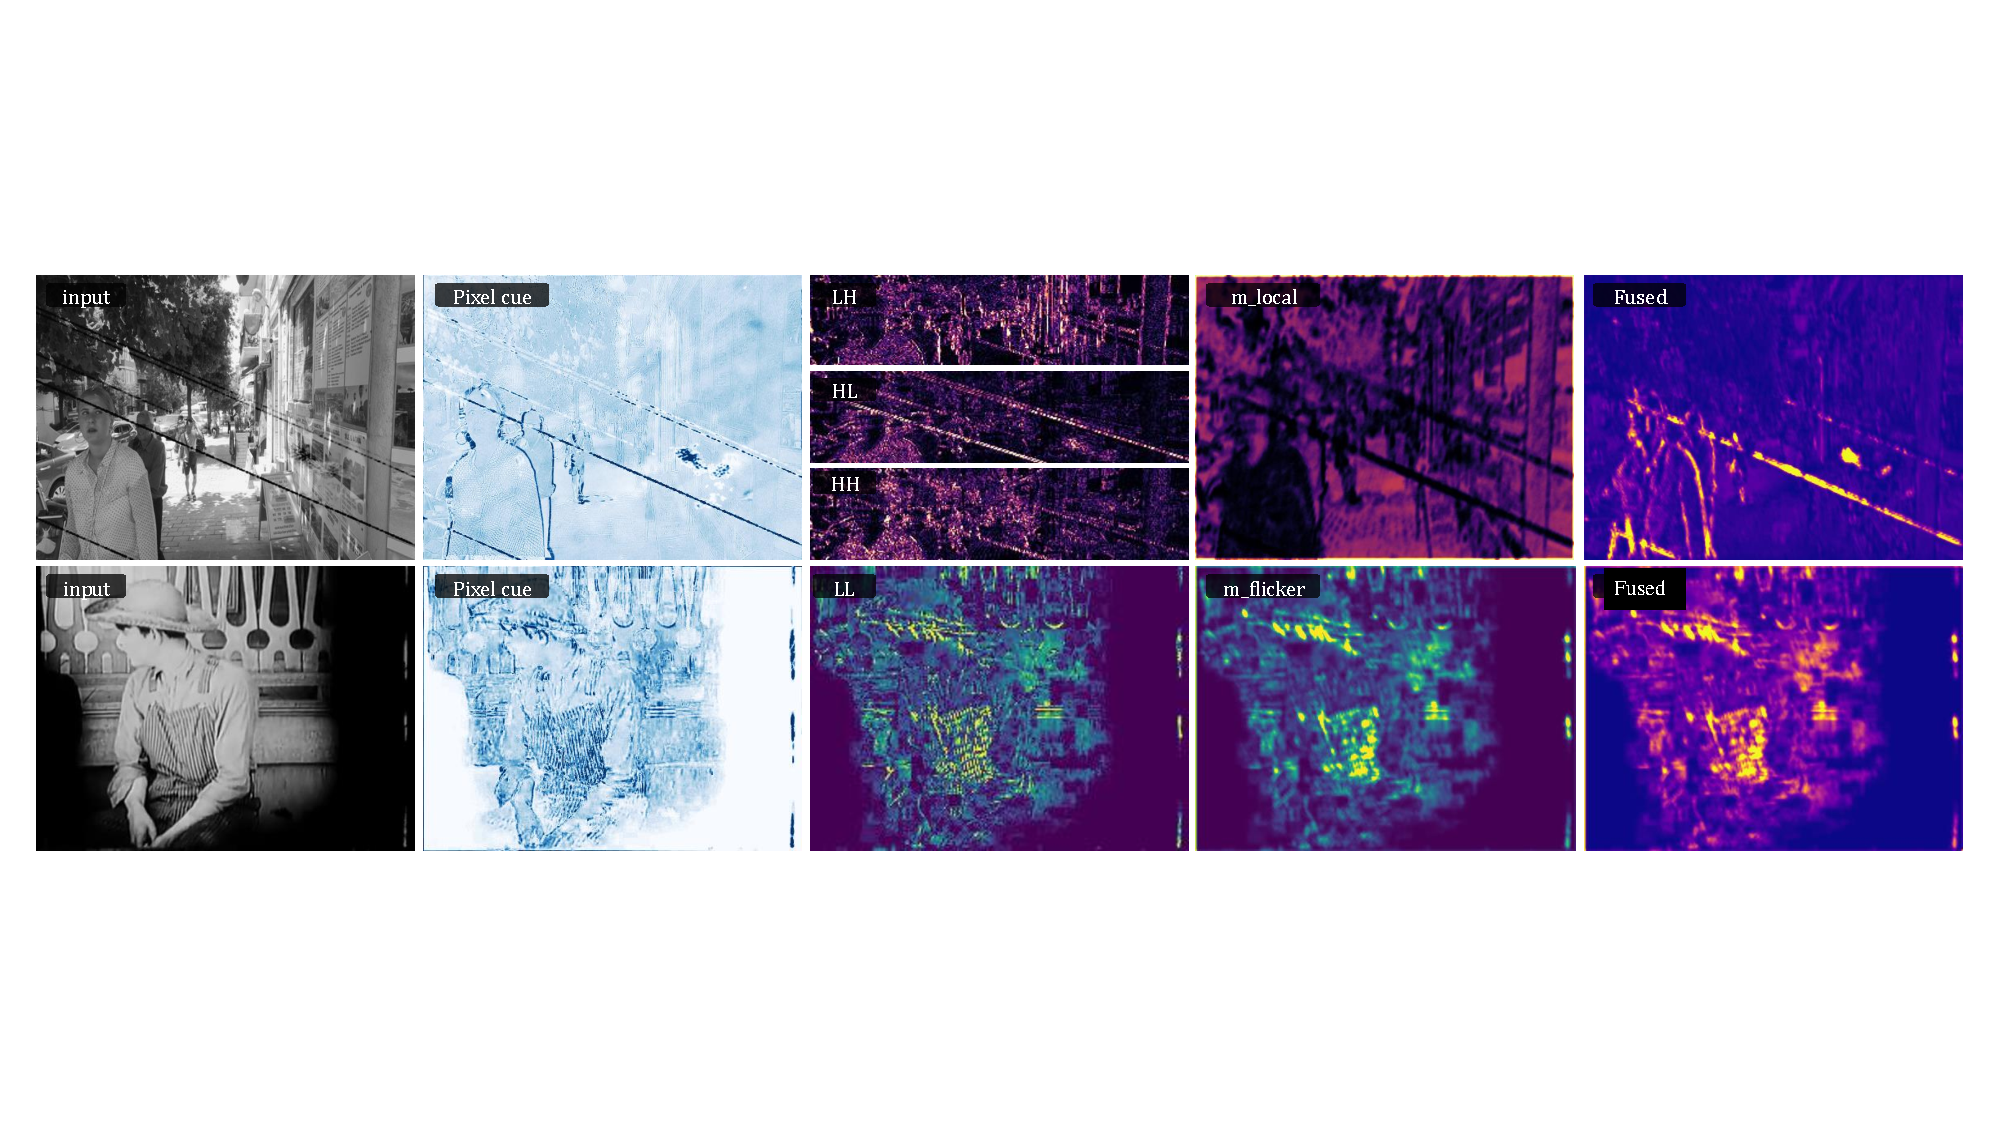
\includegraphics[width=\textwidth]{figures/Figure1.pdf}
\caption{Motivation examples for wavelet-domain degradation sensing. (a) Sparse structural damage in a synthetic validation region of interest (ROI) produces clearer Haar detail-band responses (LH/HL/HH) than the warped pixel-domain cue. (b) Brightness flicker in a real triplet from the Synthetic and Real-World Old Video (SRWOV) benchmark is emphasized by the LL temporal response and carried into the fused WaveletMask indicator. The branch-mask column reports $m_{\mathrm{local}}$ in (a) and $m_{\mathrm{flicker}}$ in (b). Except for the fixed-scale pixel cue, response and mask panels are display-normalized for visualization. The panels are qualitative motivation examples and are not used as quantitative evidence.\label{fig:motivation}}
\end{figure}

Building on this motivation, we propose \textbf{WaveletMask}, a wavelet-domain degradation detection framework for recurrent OFR. The Local High-Frequency Mask Module (LHFM; Section~\ref{subsec:local}) applies geometric-mean differencing to the Haar detail sub-bands to emphasize transient local damage. The Global Flicker Mask Module (GFM; Section~\ref{subsec:flicker}) applies a minimum-difference temporal criterion to the LL sub-band to emphasize frame-level brightness changes. The two branch masks are then combined by an element-wise maximum to form the wavelet-domain gate used for recurrent aggregation. We also evaluate learned pixel-wise fusion with the original RTN spatial indicator as an ablation. However, it is not included in the proposed model because, under the tested training recipe, it underperforms the wavelet-only gate (Table~\ref{tab:fusion_comparison}). The overall pipeline is shown in Figure~\ref{fig:pipeline}, and the two branches are detailed in Figures~\ref{fig:lhfm} and~\ref{fig:gfm}.

The main contributions are as follows:
\begin{enumerate}
    \item \textbf{WaveletMask: frequency-aware gating for recurrent OFR.} We formulate degradation sensing in the Haar wavelet domain and replace a single pixel-domain difference gate with a two-branch design that separately models high-frequency local damage and low-frequency flicker cues.

    \item \textbf{LHFM for transient structural defects.} LHFM applies geometric-mean differencing to the LH, HL, and HH sub-bands across three consecutive frames, emphasizing frame-specific scratches, dust, and other local defects while suppressing responses from persistent edges and one-sided temporal changes.

    \item \textbf{GFM for frame-level brightness instability.} GFM applies a minimum-difference criterion in the LL sub-band to detect current-frame brightness deviations relative to both temporal neighbors, yielding a dedicated cue for low-frequency flicker.

    \item \textbf{A diagnostic evaluation framework for frequency-domain degradation masks.} Under the SRWOV protocol, we establish a diagnostic evaluation framework that combines a unified re-training benchmark over ten methods with a strict paired statistical analysis against the RTN, and analyzes mask behavior through multi-seed reproducibility tests, paired clip-level significance analysis, artifact-stratified and failure-mode probes, fusion and wavelet-family ablations, and runtime measurement.
\end{enumerate}

The remainder of the paper is organized as follows. Section~\ref{sec:related_work} reviews related work. Section~\ref{sec:method} describes WaveletMask. Section~\ref{sec:results} presents synthetic, real-world, ablation, and complexity results. Section~\ref{sec:discussion} discusses interpretation, failure modes, and current limitations, including broader real-world variation and motion-related failure cases. Section~\ref{sec:conclusions} concludes the paper.


%%%%%%%%%%%%%%%%%%%%%%%%%%%%%%%%%%%%%%%%%%
\section{Related Work}\label{sec:related_work}

\subsection{Old Film Restoration Methods}

Old film restoration differs from general video restoration because archival footage often contains structured artifacts such as scratches, dust, and blotches together with photometric degradation such as flicker, grain, and fading~\cite{kokaram1998motion}. Kokaram~\cite{kokaram1998motion} summarized classical film restoration pipelines and showed that these degradations often coexist in the same sequence, but such pipelines usually treat each artifact with a separate module. Kokaram~et~al.~\cite{kokaram1995blotch} detected blotches from temporal intensity discontinuities, Joyeux~et~al.~\cite{joyeux2001scratch} tracked line scratches for reconstruction, and van Roosmalen~et~al.~\cite{vanroosmalen1999flicker} corrected brightness flicker with temporal modeling, but these methods rely on hand-crafted cues and are typically specialized to one artifact class at a time.

Wan~et~al.~\cite{wan2020bringing} proposed a domain-translation framework for old photo restoration and showed that mixed defects can be handled in a unified latent space, but the formulation is image-based and does not use temporal redundancy across frames. Iizuka and Simo-Serra~\cite{iizuka2019deepremaster} introduced DeepRemaster with 3D convolutions over spatiotemporal volumes, but the fixed receptive field makes long-range temporal aggregation less flexible. Wan~et~al.~\cite{rtn2022} proposed RTN with bidirectional recurrent propagation and a learnable soft defect mask, but the gating cue is still estimated from pixel-domain frame differences. Lin and Simo-Serra~\cite{rrtn2024} extended this line with recursive recurrent transformers, second-order grid propagation, and flow-guided deformable alignment, but the degradation indicator remains tied to spatial-domain discrepancies. Mao~et~al.~\cite{mao2025mambaofr} further incorporated Mamba-based restoration blocks and degradation-aware prompts on top of the MambaIR backbone~\cite{guo2024mambair}, but the adaptation signal is not explicitly decomposed into low-frequency and high-frequency artifact evidence.

Rota~et~al.~\cite{liu2022video_survey} reviewed deep video restoration and identified temporal propagation, motion compensation, and feature fusion as the main ingredients behind recent progress, but most existing designs are developed for generic degradations rather than archival artifacts. Chan~et~al.~\cite{chan2021basicvsr} established bidirectional recurrent propagation as an efficient temporal backbone, but the original formulation does not explicitly model degradation uncertainty. Chan~et~al.~\cite{chan2022basicvsrpp} strengthened recurrent restoration with second-order grid propagation and flow-guided deformable alignment driven by optical flow estimators such as SPyNet~\cite{ranjan2017spynet} and RAFT~\cite{teed2020raft}, but flow-guided alignment can become unreliable when severe scratches, blotches, or flicker violate motion assumptions. Vaswani~et~al.~\cite{vaswani2017attention} established the transformer formulation, and Liu~et~al.~\cite{liu2021swin} adapted it to vision through shifted-window attention, but these generic attention mechanisms do not by themselves distinguish old-film artifacts from valid scene motion. Liang~et~al.~\cite{liang2022rvrt} and Liang~et~al.~\cite{liang2024vrt} used transformer-based temporal aggregation with guided deformable attention and spatiotemporal self-attention, while Li~et~al.~\cite{li2023shiftnet} explored grouped spatial-temporal shifts for efficient restoration, but these models are still not designed around OFR-specific degradation cues. Liang~et~al.~\cite{liang2021swinir}, Zamir~et~al.~\cite{zamir2022restormer}, and Wang~et~al.~\cite{wang2021realesrgan} also improved restoration backbones on the image side, whereas Zeng~et~al.~\cite{zeng2020sttn} and Zhou~et~al.~\cite{zhou2023propainter} showed that propagation and attention are effective for video completion, but these methods are not built for dense defect-aware gating in aged film. Different from these methods, our approach keeps the recurrent OFR setting but introduces a wavelet-domain cue so that local high-frequency defects and global low-frequency flicker can be inspected separately during temporal gating.

Table~\ref{tab:method_comparison} summarizes how these representative methods differ in backbone, degradation-gating cue domain, and temporal criterion, and positions WaveletMask within this progression.

\begin{table}[H]
\caption{Method-level comparison of representative old film restoration methods, focusing on the degradation-gating cue. ``--'' denotes that the method does not use a recurrent degradation-gating cue of this type.\label{tab:method_comparison}}
\footnotesize
\begin{tabularx}{\textwidth}{lccCC}
\toprule
\textbf{Method} & \textbf{Year} & \textbf{Backbone} & \textbf{Gating Cue Domain} & \textbf{Temporal Criterion} \\
\midrule
DeepRemaster~\cite{iizuka2019deepremaster} & 2019 & 3D CNN & -- & -- \\
RTN~\cite{rtn2022} & 2022 & Bi-RNN + Swin & Pixel difference & Single-frame \\
RRTN~\cite{rrtn2024} & 2024 & Recursive RNN + Swin & Pixel difference & Bilateral \\
MambaOFR~\cite{mao2025mambaofr} & 2025 & Mamba & Latent prompt & -- \\
\textbf{WaveletMask (ours)} & 2026 & Bi-RNN + Swin & Haar wavelet sub-bands & Bilateral geometric mean / minimum \\
\bottomrule
\end{tabularx}
\normalsize
\end{table}

\subsection{Wavelet Transforms in Image and Video Restoration}

Mallat~\cite{mallat1989theory} established multiresolution wavelet analysis as a way to decompose a signal into one approximation band and multiple directional detail bands, but the theory itself does not prescribe how these sub-bands should be used for degradation detection. This decomposition is relevant to old film restoration because scratches, dust, and blotches usually produce localized high-frequency discontinuities, whereas flicker and fading mainly affect coarse luminance statistics. In this context, a single-level Haar transform provides a lightweight partition between approximation and detail responses, which is well matched to the goal of separating global brightness variation from localized defect evidence.

Liu~et~al.~\cite{liu2018mwcnn} used wavelet decomposition and inverse wavelet reconstruction as substitutes for pooling and upsampling in MWCNN, but their goal was representation learning for image restoration rather than temporal artifact detection. Huang~et~al.~\cite{huang2017wavelet} predicted wavelet coefficients for face super-resolution, and Deng~et~al.~\cite{deng2019swd} introduced wavelet-domain supervision for perception--distortion control, but these methods use wavelets in reconstruction or loss design rather than in recurrent gating.

Chen~et~al.~\cite{chen2002wavelet} investigated optical-flow estimation in the wavelet domain, and Selesnick~et~al.~\cite{selesnick2005dual} developed the dual-tree complex wavelet transform with improved directional selectivity and approximate shift invariance, but these studies were not developed for the compound and temporally varying degradations of old films. In contrast, WaveletMask operates on a single-level Haar decomposition to build a dense gating cue, using high-frequency bands to emphasize localized defects and the low-frequency band to track brightness fluctuations.

\subsection{Degradation Detection and Adaptive Mechanisms}

Li~et~al.~\cite{li2022airnet} learned a degradation representation for all-in-one image restoration and used it to guide restoration under unknown corruption, but the conditioning is performed at the latent level rather than along a dense temporal gating path. Potlapalli~et~al.~\cite{potlapalli2023promptir} introduced degradation-conditioned prompts to adapt restoration behavior across multiple corruption types, but the prompts serve as high-level control tokens instead of localized frame-wise cues. Chan~et~al.~\cite{chan2022basicvsrpp} and Liang~et~al.~\cite{liang2022rvrt} showed that adaptive temporal aggregation and alignment are crucial in video restoration, but their mechanisms are still designed for generic motion compensation and feature fusion. In the OFR setting, Wan~et~al.~\cite{rtn2022} used a representative pixel-domain indicator by comparing the current frame with flow-warped neighboring frames, and Mao~et~al.~\cite{mao2025mambaofr} further adopted prompt-style adaptation for mixed old-film degradation, but these strategies do not explicitly separate high-frequency local damage from low-frequency photometric variation.

Table~\ref{tab:feature_comparison} summarizes the conceptual difference between the two types of cues.

\begin{table}[H]
\caption{Conceptual comparison of pixel-domain and wavelet-domain degradation cues for recurrent OFR gating. The entries summarize the design motivation rather than a separate quantitative experiment.\label{tab:feature_comparison}}
\begin{tabularx}{\textwidth}{lCC}
\toprule
& \textbf{Pixel-Domain Detection} & \textbf{Wavelet-Domain Detection (Ours)} \\
\midrule
Signal domain          & Spatial intensity values & Haar wavelet sub-bands \\
High-frequency damage  & Response can be diluted when the defect footprint is spatially sparse & Detail bands often preserve sharper local responses \\
Flicker discrimination & Global intensity changes can be confounded with legitimate scene variation & The approximation band provides a more direct brightness cue \\
Temporal criterion     & Single-frame absolute difference & Bilateral geometric mean (LHFM) and minimum strategy (GFM) \\
\bottomrule
\end{tabularx}
\end{table}

Different from the global or patch-level degradation estimation used in prior work~\cite{li2022airnet,potlapalli2023promptir,mao2025mambaofr}, our approach injects a dense wavelet-domain cue into the recurrent gating path so that local defect evidence and global flicker evidence are modeled with different temporal criteria.


%%%%%%%%%%%%%%%%%%%%%%%%%%%%%%%%%%%%%%%%%%
\section{Materials and Methods}\label{sec:method}

\subsection{Problem Setup}\label{subsec:problem_setup}

WaveletMask is built on the bidirectional recurrent propagation framework of RTN~\cite{rtn2022}. Given a degraded clip $\{I_t^{\mathrm{LQ}}\}_{t=1}^{T}$ with spatial resolution $H\times W$, the goal is to reconstruct restored frames $\{I_t^{\mathrm{HQ}}\}_{t=1}^{T}$ while suppressing both local structural damage and temporal photometric artifacts. Unless otherwise stated, the batch dimension $B$ is omitted in the equations. Input frames are represented as $I_t^{\mathrm{LQ}}\in\mathbb{R}^{3\times H\times W}$, luminance frames as $I_t^{\mathrm{gray}}\in\mathbb{R}^{1\times H\times W}$, and masks as single-channel tensors in $[0,1]^{1\times H\times W}$.

In the RTN, optical flow is estimated between adjacent frames with RAFT~\cite{teed2020raft}, and a warped pixel-domain difference is used as the degradation indicator. For propagation direction $d\in\{-1,+1\}$, the directed spatial indicator is
\begin{equation}\label{eq:baseline_indicator}
    r_{t,d}^{\mathrm{spatial}} = \left|\mathcal{W}\!\left(I_{t+d}^{\mathrm{LQ}},\phi_{t+d\to t}\right)-I_t^{\mathrm{LQ}}\right|_{Y},
\end{equation}
where $\mathcal{W}(\cdot,\cdot)$ denotes flow-based warping, $\phi_{t+d\to t}$ is the estimated optical flow, and $|\cdot|_{Y}$ denotes conversion to the luminance channel after the absolute RGB difference. High indicator values encourage the gated aggregation module to rely more on current-frame evidence, whereas low values encourage reuse of propagated features.

WaveletMask replaces this motion-sensitive spatial indicator with a frame-centered wavelet-domain mask computed from bilateral temporal evidence. The detector first predicts $m_t^{\mathrm{wavelet}}$ from the current frame and its temporal neighbors, and the same mask is then injected into both propagation directions:
\begin{equation}\label{eq:gate_mask}
    m_{t,d}^{\mathrm{gate}} = m_t^{\mathrm{wavelet}}, \quad d\in\{-1,+1\}.
\end{equation}
Using a shared gate mask for $d\in\{-1,+1\}$ matches the implementation and reflects the fact that the wavelet detector is anchored at frame $t$ rather than at a specific propagation direction. In the proposed model, $m_t^{\mathrm{wavelet}}$ is obtained from LHFM and GFM followed by element-wise maximum fusion. Learned variants that additionally combine the RTN spatial indicator with the wavelet mask are evaluated only as ablations in Appendix~\ref{subsec:fusion_analysis} and are not part of the final architecture.

\subsection{Pipeline Overview}\label{subsec:overview}

Figure~\ref{fig:pipeline} summarizes the final WaveletMask pipeline. For each frame, the WaveletNoiseMask block pre-computes a wavelet-domain gate mask from the current frame and its two temporal neighbors, and the resulting $m_t^{\mathrm{wavelet}}$ is injected directly into the forward and backward recurrent gates in Equation~\eqref{eq:gate_mask}. The restoration backbone, bidirectional propagation schedule, and training losses remain identical to RTN; only the gate input is changed.

\begin{figure}[t]
\centering
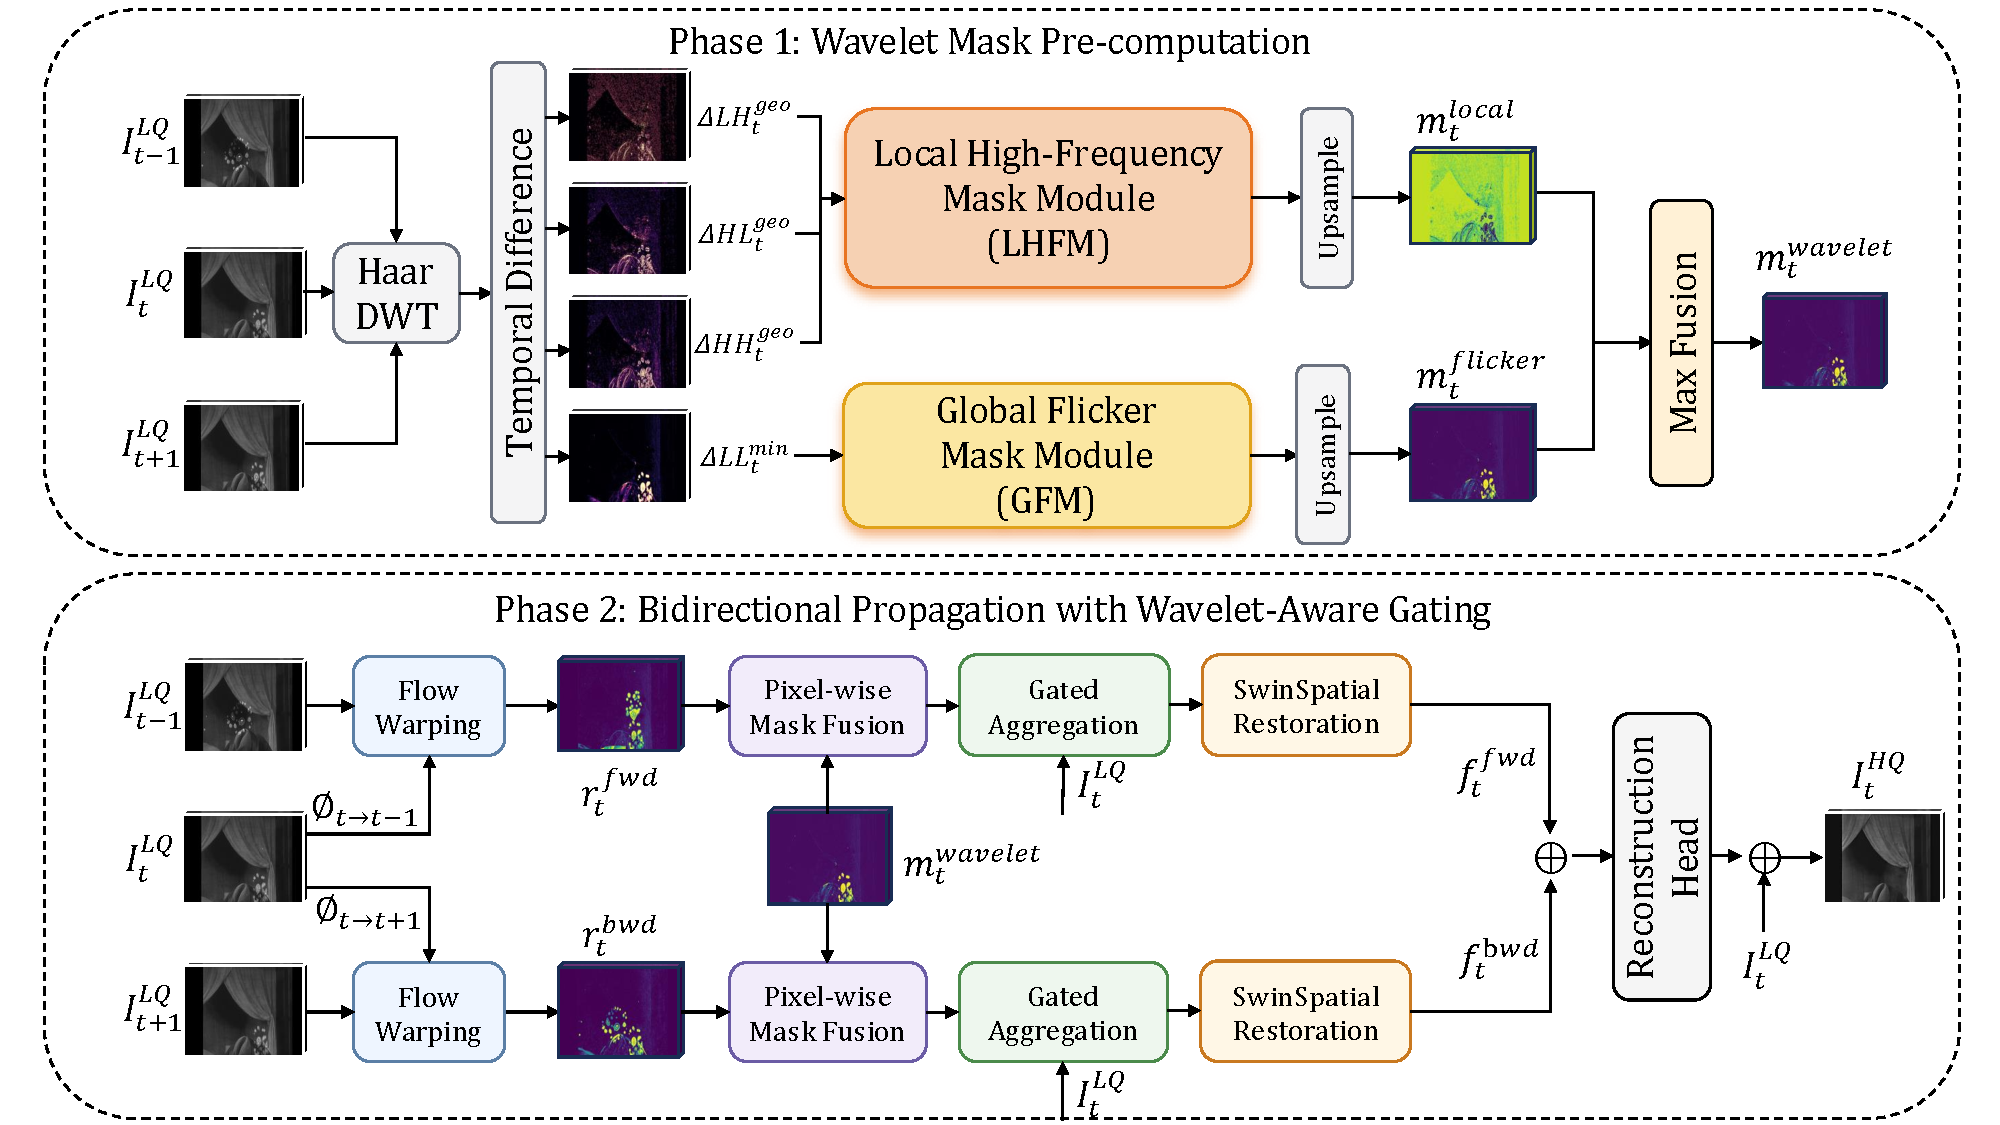
\includegraphics[width=\textwidth]{figures/Figure2.pdf}
\caption{Overview of the final WaveletMask pipeline. The WaveletNoiseMask module pre-computes the branch-max wavelet mask $m_t^{\mathrm{wavelet}}$ from neighboring frames, and the resulting mask is injected directly into the forward and backward recurrent gates. Learned CNN fusion variants that additionally use the RTN spatial indicator are ablated in Table~\ref{tab:fusion_comparison} and are not part of the proposed model.\label{fig:pipeline}}
\end{figure}

Unlike the flow-guided propagation path in RTN, the wavelet detector intentionally operates on raw temporal neighbors instead of motion-compensated ones. An auxiliary code path includes an optional flow-compensated wavelet variant, but this switch is disabled in the proposed model because a small pixel-domain misregistration perturbs multiple LL/LH/HL/HH coefficients after the discrete wavelet transform, thereby amplifying optical-flow errors into structured false responses near motion boundaries. For the same reason, the proposed model fixes a single-level Haar decomposition; alternative wavelet families and learned fusion variants are reserved for ablation-only experiments.

The recurrent aggregation step can be written as
\begin{equation}\label{eq:gated_agg}
    f_t^{\mathrm{agg}} = \mathrm{GatedAgg}\!\left(f_{\mathrm{prop}},I_t^{\mathrm{LQ}},m_{t,d}^{\mathrm{gate}}\right),
\end{equation}
where $m_{t,d}^{\mathrm{gate}}$ is broadcast along the feature-channel dimension. The reconstruction head follows the original RTN contract:
\begin{equation}\label{eq:reconstruction}
    I_t^{\mathrm{HQ}} = \tanh\!\left(\mathrm{Upsample}\!\left([f_t^{\mathrm{bwd}},f_t^{\mathrm{fwd}}]\right)+I_t^{\mathrm{LQ}}\right).
\end{equation}
Because the wavelet mask is pre-computed before recurrent propagation and the final fusion is parameter-free, the proposed variant changes only the gate input while leaving the restoration backbone, losses, and propagation structure unchanged.

\subsection{Local High-Frequency Mask Module (LHFM)}\label{subsec:local}

Unlike pixel-domain differences that entangle thin defects with motion boundaries and warping residuals, LHFM isolates transient local corruption by measuring bilateral consistency in the wavelet detail sub-bands. Figure~\ref{fig:lhfm} shows the module architecture.

\begin{figure}[t]
\centering
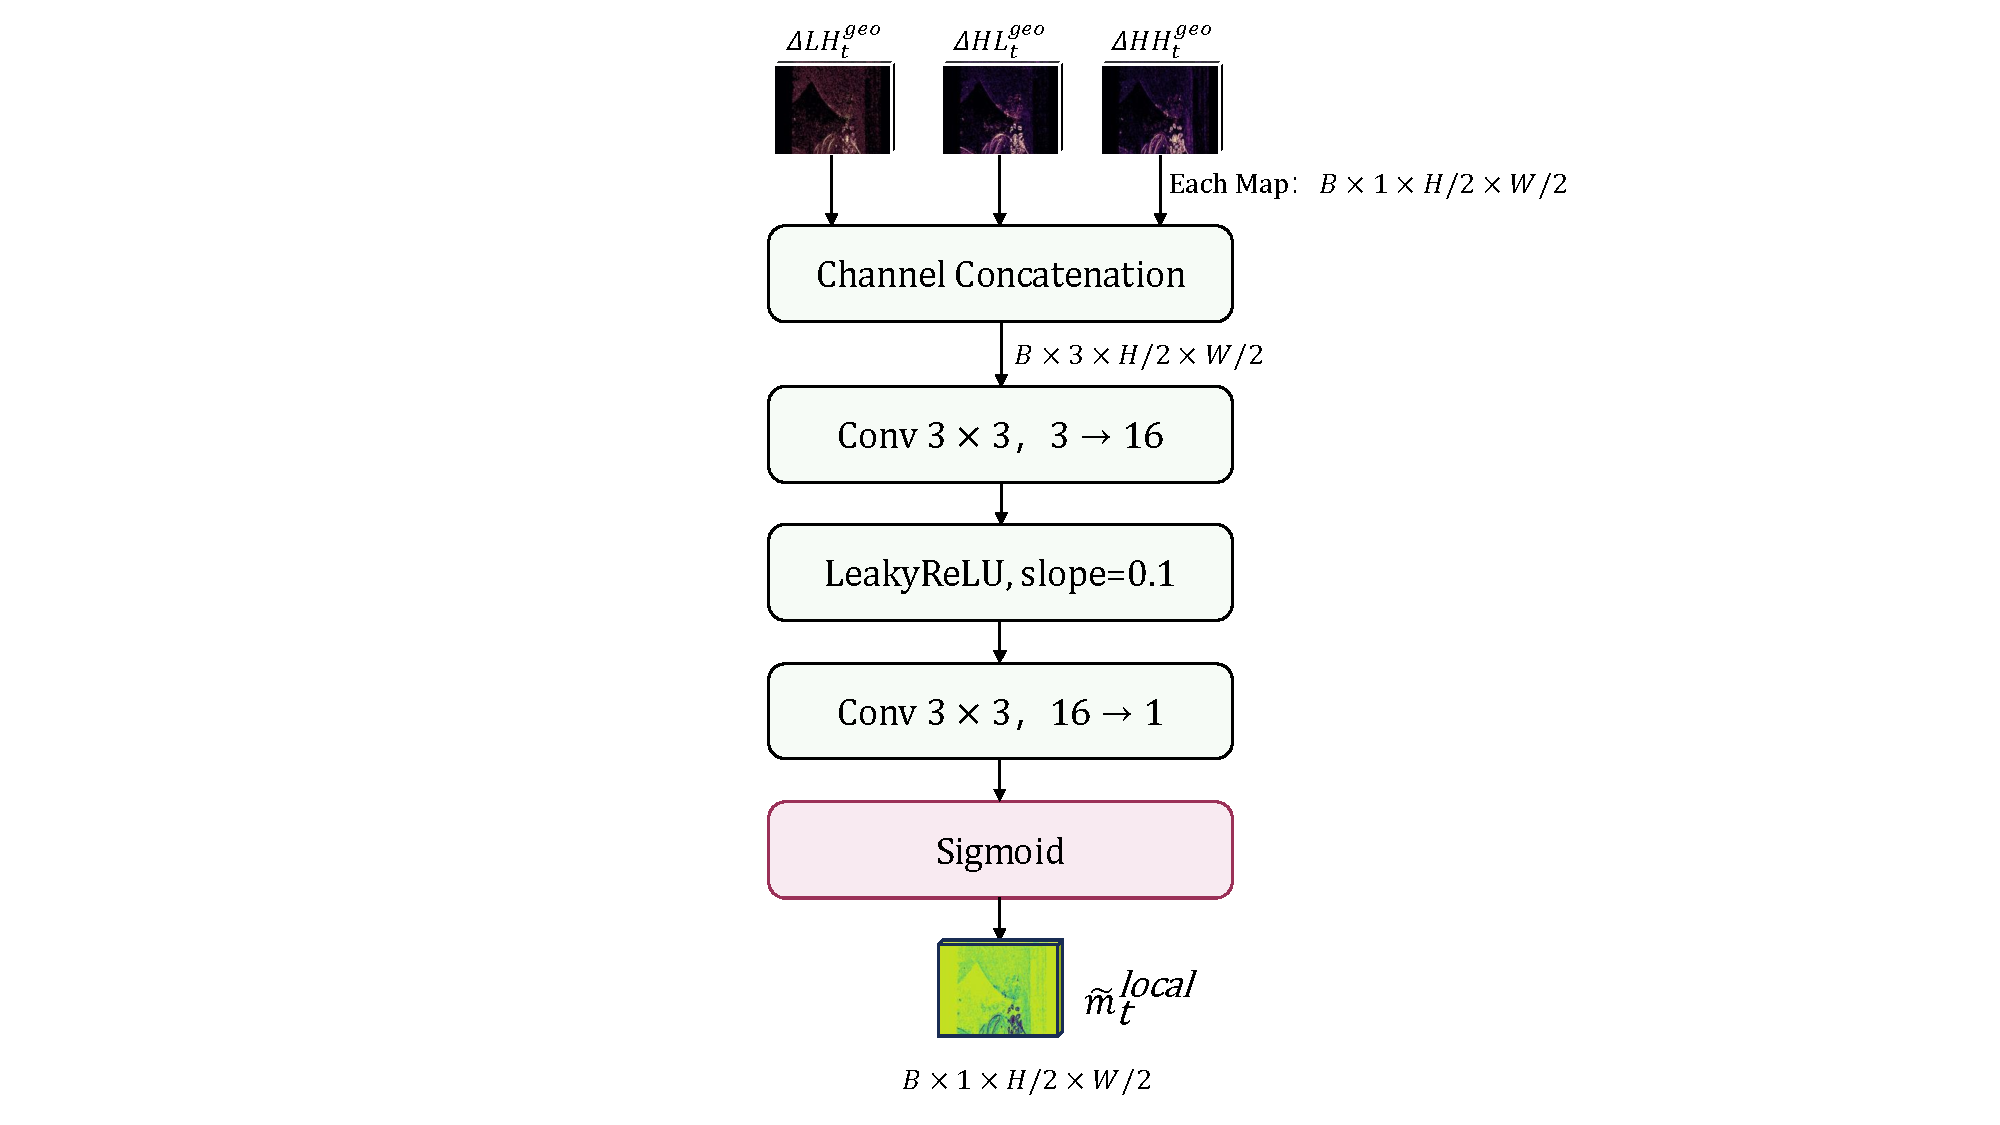
\includegraphics[width=\textwidth]{figures/Figure3.pdf}
\caption{LHFM architecture. Geometric-mean temporal differences from the LH, HL, and HH detail sub-bands are concatenated and processed by \texttt{high\_freq\_conv}, consisting of a 3$\times$3 3$\to$16 convolution, LeakyReLU, a 3$\times$3 16$\to$1 convolution, and sigmoid activation. The half-resolution output $\tilde{m}_t^{\mathrm{local}}\in[0,1]^{1\times H/2\times W/2}$ is bilinearly upsampled before fusion.\label{fig:lhfm}}
\end{figure}

Each RGB frame is first converted to luminance using the BT.601 transform, $I_t^{\mathrm{gray}}=0.299R+0.587G+0.114B$, and is then decomposed by a single-level Haar DWT:
\begin{equation}\label{eq:haar_dwt}
    \{\mathrm{LL}_t,\mathrm{LH}_t,\mathrm{HL}_t,\mathrm{HH}_t\}=\mathrm{HaarDWT2d}(I_t^{\mathrm{gray}}).
\end{equation}
Here, $\mathrm{LL}_t$ denotes the low-frequency approximation, while $\mathrm{LH}_t$, $\mathrm{HL}_t$, and $\mathrm{HH}_t$ denote the horizontal, vertical, and diagonal detail coefficients, respectively. The proposed model uses fixed $2\times2$ Haar analysis filters normalized by $1/2$, so the transform introduces no learnable parameters.

To suppress one-sided temporal residuals, LHFM requires simultaneous disagreement with both temporal neighbors. For each high-frequency sub-band $S\in\{\mathrm{LH},\mathrm{HL},\mathrm{HH}\}$, the bilateral response is computed as
\begin{equation}\label{eq:geomean}
    d_t^{S}=\sqrt{|S_t-S_{t^-}|\,|S_t-S_{t^+}|+\epsilon},
\end{equation}
where $t^-$ and $t^+$ denote the previous and next neighbors for non-boundary frames, and $\epsilon=10^{-8}$ is used for numerical stability. The geometric mean behaves like a bilateral ``and'' operator: if either temporal difference is small, the overall response remains small. Consequently, one-sided motion or warping residuals are attenuated, whereas a transient scratch or dust particle that differs from both neighbors produces a strong activation. Boundary frames do not have bilateral temporal evidence and are assigned zero wavelet masks. This design is effective for single-frame defects, but when a scratch persists across three or more consecutive frames at nearly the same image-plane position ($S_{t-1}\approx S_t\approx S_{t+1}$), both temporal differences vanish and $d_t^S\to 0$, suppressing the LHFM response (see Section~\ref{subsec:response_analysis} and Table~\ref{tab:persistent_scratch_probe}).

The three directional responses are then aggregated by a lightweight prediction head:
\begin{equation}\label{eq:local_mask}
    \tilde{m}_t^{\mathrm{local}}=\sigma\!\left(\mathrm{Conv}_{16\to1}\!\left(\mathrm{LeakyReLU}\!\left(\mathrm{Conv}_{3\to16}\!\left([d_t^{\mathrm{LH}},d_t^{\mathrm{HL}},d_t^{\mathrm{HH}}]\right)\right)\right)\right),
\end{equation}
where $\sigma$ denotes the sigmoid activation and $[\cdot]$ denotes channel-wise concatenation. The resulting half-resolution prediction is bilinearly upsampled to the image resolution:
\begin{equation}\label{eq:local_mask_up}
    m_t^{\mathrm{local}}=\mathrm{Up}(\tilde{m}_t^{\mathrm{local}}), \quad m_t^{\mathrm{local}}\in[0,1]^{1\times H\times W},
\end{equation}
where $\mathrm{Up}(\cdot)$ denotes bilinear upsampling.

\subsection{Global Flicker Mask Module (GFM)}\label{subsec:flicker}

Unlike pixel-domain differences that are dominated by edges, texture, and local motion, GFM captures frame-level photometric instability by measuring bilateral low-frequency deviations on the LL sub-band. Figure~\ref{fig:gfm} shows the module architecture.

After obtaining the LL coefficients, we compute the forward and backward low-frequency deviations as
\begin{equation}\label{eq:flicker_diff}
    d_t^{\mathrm{fwd}}=|\mathrm{LL}_t-\mathrm{LL}_{t^-}|,\quad d_t^{\mathrm{bwd}}=|\mathrm{LL}_t-\mathrm{LL}_{t^+}|.
\end{equation}
GFM then enforces bilateral agreement through a minimum operator:
\begin{equation}\label{eq:flicker_min}
    d_t^{\mathrm{flicker}}=\min(d_t^{\mathrm{fwd}},d_t^{\mathrm{bwd}}).
\end{equation}
The minimum rule is used instead of an average because a genuine flicker event should increase both forward and backward LL differences. If only one direction is large, the response is limited to the smaller value, which reduces sensitivity to one-sided brightness changes. At the same time, abrupt scene cuts, flashes, and other broad illumination changes can also elevate both LL differences. These failure modes are quantified in Table~\ref{tab:gfm_failure_probe} and discussed in Section~\ref{subsec:response_analysis}.

\begin{figure}[H]
\centering
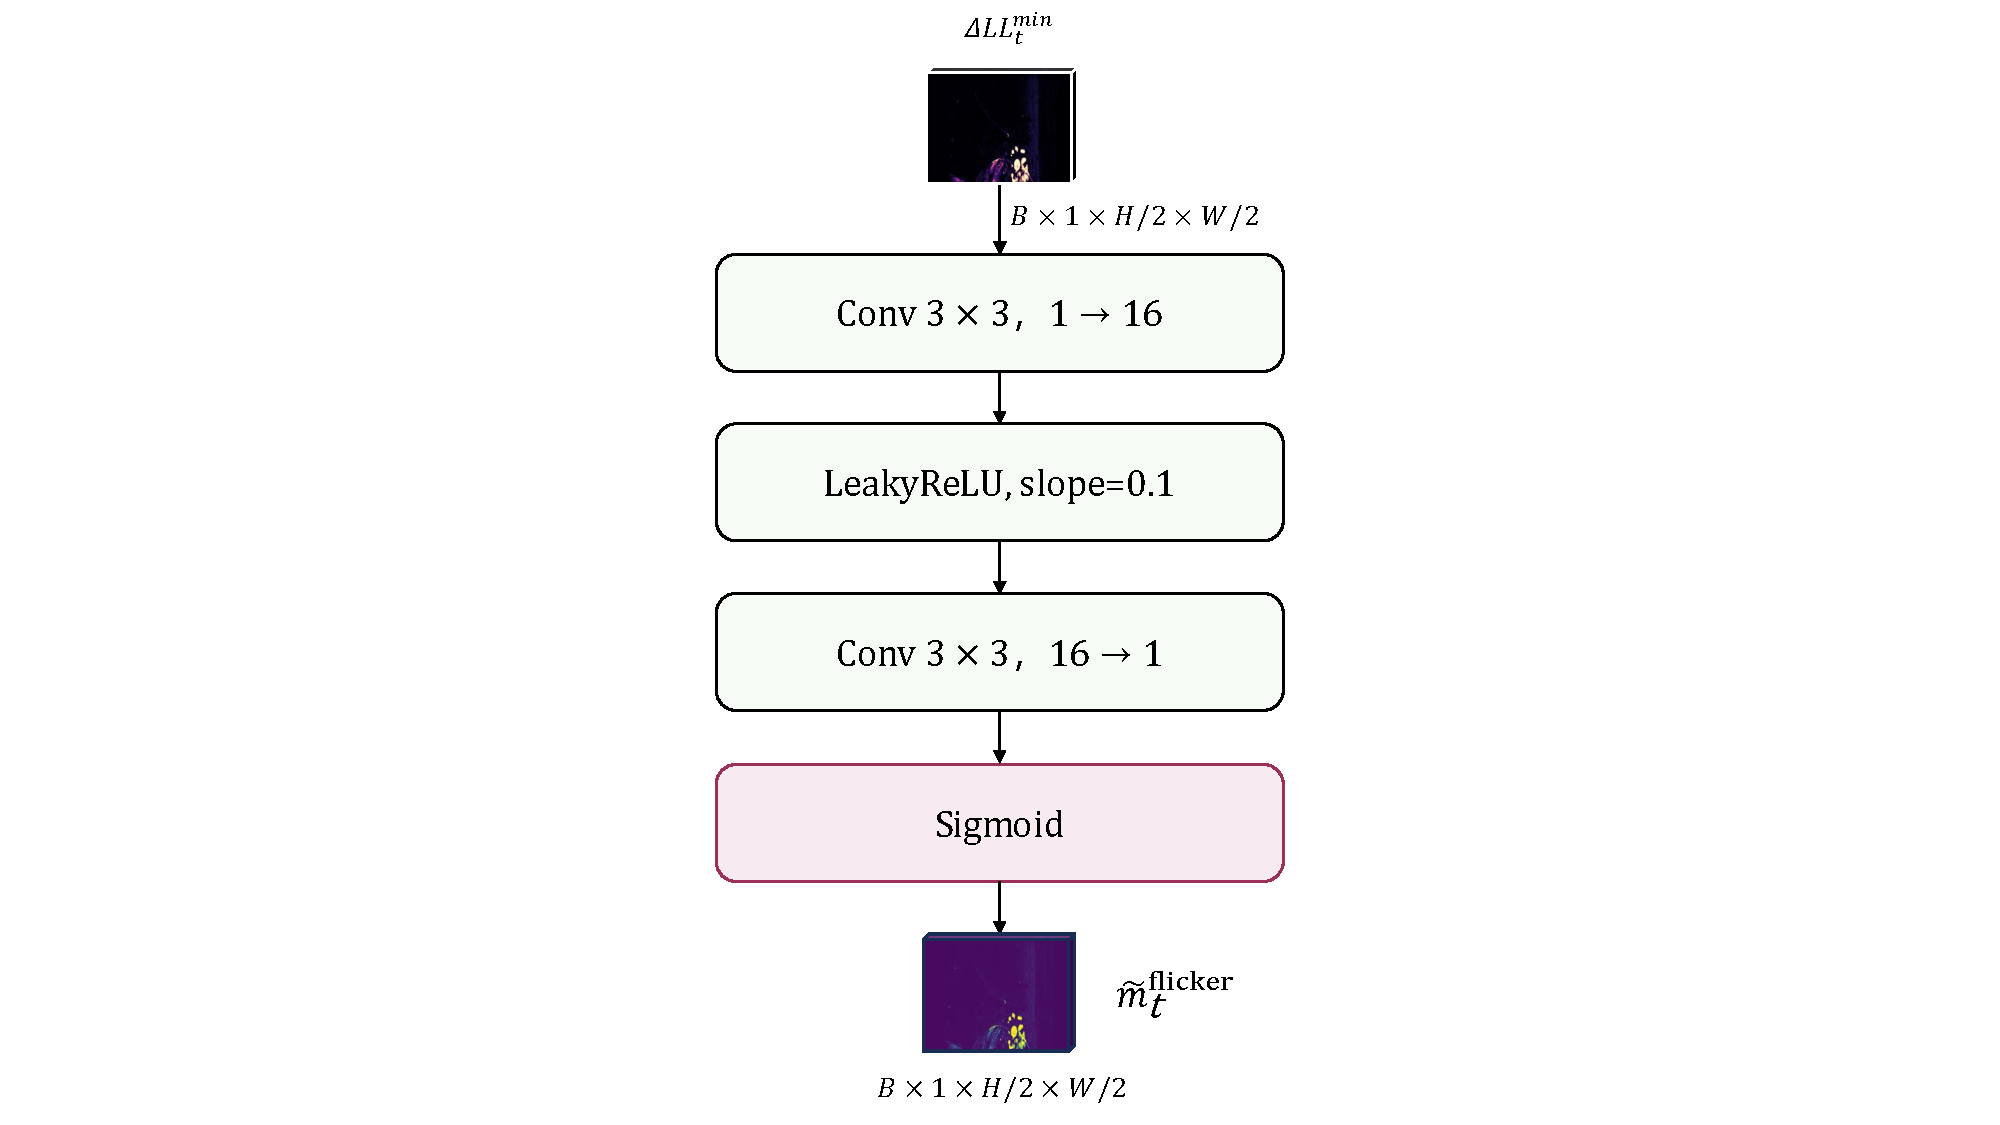
\includegraphics[width=\textwidth]{figures/Figure4.pdf}
\caption{GFM architecture. The minimum LL temporal response is processed by \texttt{low\_freq\_conv}, consisting of a 3$\times$3 1$\to$16 convolution, LeakyReLU, a 3$\times$3 16$\to$1 convolution, and sigmoid activation. The half-resolution output $\tilde{m}_t^{\mathrm{flicker}}\in[0,1]^{1\times H/2\times W/2}$ is bilinearly upsampled before fusion.\label{fig:gfm}}
\end{figure}

The low-frequency response is decoded by a second lightweight prediction head:
\begin{equation}\label{eq:flicker_mask}
    \tilde{m}_t^{\mathrm{flicker}}=\sigma\!\left(\mathrm{Conv}_{16\to1}\!\left(\mathrm{LeakyReLU}\!\left(\mathrm{Conv}_{1\to16}(d_t^{\mathrm{flicker}})\right)\right)\right),
\end{equation}
followed by bilinear upsampling to the original resolution:
\begin{equation}\label{eq:flicker_mask_up}
    m_t^{\mathrm{flicker}}=\mathrm{Up}(\tilde{m}_t^{\mathrm{flicker}}), \quad m_t^{\mathrm{flicker}}\in[0,1]^{1\times H\times W}.
\end{equation}

\subsection{Mask Fusion and Integration}\label{subsec:integration}

Unlike pixel-domain differences that collapse local scratches and global luminance shifts into a single motion-sensitive residual, the integration stage preserves whichever wavelet branch provides the stronger evidence at each pixel. As further clarified in Section~\ref{subsec:response_analysis}, LHFM and GFM are complementary rather than redundant, so the fusion rule should avoid attenuating a decisive single-branch response.

WaveletMask therefore uses a branch-level maximum operation:
\begin{equation}\label{eq:wavelet_mask}
    m_t^{\mathrm{wavelet}}=\max(m_t^{\mathrm{local}},m_t^{\mathrm{flicker}}).
\end{equation}
The element-wise maximum treats local structural damage and global flicker as alternative degradation evidence: if either branch fires, the wavelet mask is activated. This choice also matches the implementation exactly, where $\max(\cdot,\cdot)$ is used directly after the two mask heads. Compared with learned convex fusion, this rule preserves a strong activation from either branch instead of averaging it with a weak companion response. The ablation results in Table~\ref{tab:fusion_comparison} further show that parameter-free max fusion is preferable to learned PixelWiseMaskFusion, which supports the final design choice.

The complete detector consists of the fixed Haar DWT and two lightweight CNN heads, introducing only 898 learnable detector parameters. By contrast, the learned PixelWiseMaskFusion ablation adds 14,497 additional fusion parameters and also mixes in the RTN spatial indicator. These learned spatial--wavelet fusion variants are therefore treated as ablations rather than components of the final WaveletMask model.

\subsection{Response Analysis}\label{subsec:response_analysis}

To clarify the design rationale and boundary conditions of LHFM and GFM, we analyze several canonical temporal patterns.

\textbf{Local high-frequency response.} Equation~\eqref{eq:geomean} is designed to respond strongly only when the current high-frequency coefficient differs from both temporal neighbors. For a single-frame transient scratch at time $t$ ($S_{t-1}=0,\;S_t>0,\;S_{t+1}=0$), both terms under the geometric mean are large, producing the intended strong $d_t^S$ response. If only one directional difference is elevated, the product remains limited, which explains why the geometric mean suppresses one-sided motion or warping residuals more effectively than a simple sum or average. Conversely, for a persistent fixed scratch spanning $\geq$3 frames ($S_{t-1}\approx S_t\approx S_{t+1}$), both temporal differences vanish and $d_t^S\to0$, suppressing the LHFM response. This is an inherent boundary condition of the bilateral design: persistent image-plane-fixed scratches are progressively attenuated with increasing persistence length (46\% suppression at $L=2$, 65\% at $L\geq3$; see Table~\ref{tab:persistent_scratch_probe}). Drifting scratches that shift spatially between frames break the equality condition and are therefore not suppressed in the same way.

\textbf{Global flicker response.} Equation~\eqref{eq:flicker_min} similarly enforces bilateral agreement, but on the low-frequency LL component. A valid flicker event causes both forward and backward LL differences to increase, so the minimum remains high; this is why the minimum rule is better aligned with frame-level flicker than an average that can be dominated by a single-sided deviation. However, scene cuts and exposure flashes also produce bilateral LL elevation. In our probes, a scene cut yields $2.35\times$ baseline activation, and a flash yields $10.41\times$ (Table~\ref{tab:gfm_failure_probe}). A luminance-difference guard can suppress 61\% of scene-cut and 95\% of flash false responses, but it is not integrated into the current model in order to keep the proposed detector lightweight and scope-consistent.

Taken together, these complementary response patterns explain the integration strategy in Section~\ref{subsec:integration}: the final gate should preserve the stronger local or global cue at each pixel, rather than learn an averaging rule that may dilute a decisive single-branch response.

\subsection{Training Objective}\label{subsec:training}

Training follows the RTN protocol~\cite{rtn2022}. The total objective is
\begin{equation}\label{eq:loss_total}
    \mathcal{L}_{\mathrm{total}}=\mathcal{L}_{\mathrm{pix}}+\lambda_{\mathrm{perc}}\mathcal{L}_{\mathrm{perc}}+\lambda_{\mathrm{gan}}\mathcal{L}_{\mathrm{gan}},
\end{equation}
where $\mathcal{L}_{\mathrm{pix}}$ is an $L_1$ reconstruction loss, $\mathcal{L}_{\mathrm{perc}}$ is a VGG-based perceptual loss~\cite{johnson2016perceptual,simonyan2014vgg}, and $\mathcal{L}_{\mathrm{gan}}$ is a non-saturating adversarial loss~\cite{goodfellow2014gan}. The weights are $\lambda_{\mathrm{perc}}=1.0$ and $\lambda_{\mathrm{gan}}=0.01$, following RTN~\cite{rtn2022}. No explicit mask supervision is used; the wavelet branches and the restoration backbone are optimized only through the restoration losses. This choice preserves compatibility with the baseline training loop, but it also limits how strongly the learned masks can be interpreted as ground-truth artifact segmentations.


%%%%%%%%%%%%%%%%%%%%%%%%%%%%%%%%%%%%%%%%%%
\section{Experiments}\label{sec:results}

This section describes the experimental setup, compares WaveletMask with state-of-the-art methods on synthetic and real-world data, presents the ablation study, and analyzes computational complexity. Detailed statistical-reliability analyses, robustness and cross-content generalization studies, detector diagnostic probes, and full ablation sweeps are reported in Appendices~\ref{app:stats}--\ref{app:complexity_details}.

\subsection{Datasets}

Experiments are conducted on the Synthetic and Real-World Old Video (SRWOV) benchmark introduced with MambaOFR~\cite{mao2025mambaofr}. The synthetic split provides paired ground truth and is used for full-reference evaluation. The real-world split contains archival clips without paired ground truth and is used for no-reference metrics and qualitative comparisons.

Training uses the REDS training split~\cite{nah2019reds}. Clean REDS frames are degraded on the fly with the synthetic film degradation pipeline used by RTN~\cite{rtn2022}, including scratches, dust, blotches, flicker, and grain. The SRWOV synthetic test set contains 30 clips rendered from held-out REDS sequences, and the SRWOV real-world set contains 216 archival clips. Unless otherwise noted, the quantitative results below are reported within this SRWOV protocol. Qualitative figures are illustrative; statistical claims rest on the unified re-training benchmark in Table~\ref{tab:literature_context} and the strict paired controlled analysis in Appendix~\ref{app:stats}.

\subsection{Implementation Details}\label{subsec:implementation}

RTN and all WaveletMask variants are trained with the same recipe. We use Adam~\cite{kingma2015adam} with $\beta_1=0.9$, $\beta_2=0.99$, initial learning rate $2\times10^{-4}$, and a MultiStep schedule with milestones at 50K, 100K, and 150K iterations. Training uses 200K iterations, seven input frames, $256\times256$ crops, and batch size~1 per GPU. The configuration sets \texttt{fix\_flow\_iters}=0.0005, so the RAFT~\cite{teed2020raft} optical-flow estimator is effectively trained jointly from the start rather than frozen for a 500-iteration warm-up. Experiments are implemented in PyTorch with the BasicSR toolbox~\cite{wang2022basicsr}; inference is performed at full resolution. The strict paired controlled comparison against the RTN (Appendix~\ref{app:stats}) is reported for seed 2021, and a three-seed Y-channel re-test is reported separately to assess seed stability.

\subsection{Evaluation Metrics}\label{subsec:metrics}

Following common practice in old film restoration~\cite{rtn2022,rrtn2024,mao2025mambaofr}, we adopt three complementary groups of metrics. (1) On the synthetic split with paired ground truth, we report the fidelity metrics PSNR and SSIM~\cite{wang2004ssim} together with the perceptual metrics LPIPS~\cite{zhang2018lpips} and DISTS~\cite{ding2020dists}; all full-reference metrics are computed under the Y-channel protocol. (2) On the real-world split without ground truth, we report the no-reference metrics NIQE~\cite{mittal2013niqe}, BRISQUE~\cite{mittal2012brisque}, and CLIPIQA+~\cite{wang2023clipiqa}; these no-reference metrics, together with the qualitative comparisons, constitute the primary real-world evidence. (3) To quantify statistical reliability, we report clip-level bootstrap confidence intervals, two-sided paired permutation tests, and a three-seed re-test for the paired controlled comparison; the complete statistics are provided in Appendix~\ref{app:stats}.

For completeness, the two primary full-reference metrics are defined as follows. Given a restored luminance frame $\hat{I}$ and its ground truth $I$ with $N$ pixels, the peak signal-to-noise ratio (PSNR) is
\begin{equation}
\mathrm{PSNR}(\hat{I}, I) = 10\log_{10}\frac{L^{2}}{\frac{1}{N}\sum_{i=1}^{N}(\hat{I}_{i}-I_{i})^{2}},
\end{equation}
where $L$ is the maximum possible pixel value, and the structural similarity index (SSIM) is
\begin{equation}
\mathrm{SSIM}(\hat{I}, I) = \frac{(2\mu_{\hat{I}}\mu_{I}+c_{1})(2\sigma_{\hat{I}I}+c_{2})}{(\mu_{\hat{I}}^{2}+\mu_{I}^{2}+c_{1})(\sigma_{\hat{I}}^{2}+\sigma_{I}^{2}+c_{2})},
\end{equation}
where $\mu_{\cdot}$ and $\sigma_{\cdot}$ denote local means and standard deviations, $\sigma_{\hat{I}I}$ is the local covariance, and $c_{1},c_{2}$ are small stabilizing constants. The perceptual metrics LPIPS and DISTS and the no-reference metrics NIQE, BRISQUE, and CLIPIQA+ follow the definitions in their original references.

\subsection{Comparison with State-of-the-Art Methods}\label{subsec:sota}

We compare WaveletMask with representative methods from three categories: old photo restoration applied per frame (OldPhoto~\cite{wan2020bringing}, DeOldify~\cite{jantic2019deoldify}), general video restoration (ShiftNet~\cite{li2023shiftnet}, VRT~\cite{liang2024vrt}, RVRT~\cite{liang2022rvrt}), and dedicated old film restoration (DeepRemaster~\cite{iizuka2019deepremaster}, RTN~\cite{rtn2022}, RRTN~\cite{rrtn2024}, MambaOFR~\cite{mao2025mambaofr}). All ten methods, including WaveletMask, were re-trained and re-evaluated on the same SRWOV synthetic split under one unified benchmark pipeline, so they are directly comparable; in addition, a strict paired controlled analysis against RTN---which shares the backbone, training data, degradation pipeline, and metric scripts with WaveletMask---is reported in Appendix~\ref{app:stats}.

\subsubsection{Quantitative Comparison on Synthetic Data}\label{subsec:sota_quant}

\begin{table}[H]
\caption{Unified re-training benchmark on the SRWOV synthetic split (30 clips, Y-channel protocol), listed in chronological order of publication with the proposed WaveletMask in the last row. All methods, including WaveletMask, were re-trained and re-evaluated by us under one unified benchmark pipeline, so the rows are directly comparable. Best results are in \textcolor{red}{red} and second-best results in \textcolor{blue}{blue}.\label{tab:literature_context}}
\footnotesize
\begin{tabularx}{\textwidth}{lcCCCC}
\toprule
\textbf{Method} & \textbf{Year} & \textbf{PSNR$\uparrow$} & \textbf{SSIM$\uparrow$} & \textbf{LPIPS$\downarrow$} & \textbf{DISTS$\downarrow$} \\
\midrule
DeepRemaster~\cite{iizuka2019deepremaster}  & 2019 & 25.0590 & \textcolor{red}{0.9185} & 0.1108 & 0.0895 \\
DeOldify~\cite{jantic2019deoldify}          & 2019 & 23.2197 & 0.8923 & 0.2775 & 0.1260 \\
OldPhoto~\cite{wan2020bringing}             & 2020 & 24.6174 & 0.8524 & 0.2252 & 0.1144 \\
RTN~\cite{rtn2022}                          & 2022 & 25.8514 & 0.8869 & 0.1214 & 0.0862 \\
RVRT~\cite{liang2022rvrt}                   & 2022 & 22.4317 & 0.8710 & 0.1655 & 0.1078 \\
ShiftNet~\cite{li2023shiftnet}              & 2023 & 21.4817 & 0.8234 & 0.2030 & 0.1303 \\
RRTN~\cite{rrtn2024}                        & 2024 & 24.1450 & 0.9006 & 0.1082 & \textcolor{red}{0.0668} \\
VRT~\cite{liang2024vrt}                     & 2024 & 22.3866 & 0.8631 & 0.1750 & 0.1087 \\
MambaOFR~\cite{mao2025mambaofr}             & 2025 & \textcolor{blue}{25.9938} & \textcolor{blue}{0.9059} & \textcolor{red}{0.0815} & \textcolor{blue}{0.0822} \\
\midrule
\textbf{WaveletMask (ours)}                 & 2026 & \textcolor{red}{26.6017} & 0.8951 & \textcolor{blue}{0.0891} & 0.0831 \\
\bottomrule
\end{tabularx}
\normalsize
\end{table}

Table~\ref{tab:literature_context} reports the unified re-training benchmark over ten methods. Under this single comparable protocol, WaveletMask attains the best PSNR (26.60~dB, $+0.61$~dB over the strongest competitor MambaOFR) and the second-best LPIPS. On DISTS it is essentially tied with the second-best method (0.0831 vs.\ 0.0822 for MambaOFR), whereas on SSIM it sits mid-table, behind the perception-oriented methods DeepRemaster, MambaOFR, and RRTN. The benchmark thus indicates a clear fidelity advantage together with competitive perceptual quality rather than uniform dominance across metrics: among the recent dedicated baselines, MambaOFR remains the strongest on the structural and perceptual scores, while WaveletMask leads on PSNR at a fraction of the detector parameter cost (Section~\ref{subsec:complexity}). Beyond this benchmark, a strict paired controlled comparison against the RTN isolates the contribution of the proposed gate: WaveletMask improves PSNR by $+0.45$~dB, all four paired clip-level gains are statistically significant under two-sided permutation tests ($p\le1.5\times10^{-3}$), and a three-seed re-test confirms that the advantage persists with markedly higher stability than the baseline (26.22$\pm$0.37 vs. 24.56$\pm$1.67~dB PSNR; Appendix~\ref{app:stats}, Tables~\ref{tab:same_protocol_main}--\ref{tab:three_seed_summary}). The WaveletMask unified-benchmark entry (26.6017~dB) differs slightly from this paired value (26.6125~dB), and the unified-benchmark RTN entry (25.8514~dB) likewise differs from the paired-protocol RTN (26.1648~dB; Table~\ref{tab:ablation_core}), because the two protocols use different training checkpoints and metric configurations. The gain is not confined to a single degradation mode: it is positive in all artifact-dominant strata, remains stable across motion and occlusion terciles, and transfers to unseen DAVIS content in PSNR, LPIPS, and DISTS under the same degradation pipeline (Appendix~\ref{app:robustness}).

\subsubsection{No-Reference Comparison on Real-World Data}\label{subsec:realworld}

Real-world SRWOV clips do not have paired ground truth, so we report them separately from the full-reference synthetic results. Table~\ref{tab:realworld_literature} reports our unified-benchmark no-reference scores for all ten methods together with the degraded-input anchor on the 216-clip SRWOV real-world split. A no-reference ablation over the RTN/LHFM/GFM variants under the strict paired protocol (Appendix~\ref{app:stats}) is provided in Appendix~\ref{app:complexity_details} (Table~\ref{tab:realworld_variants}).

\begin{table}[H]
\caption{No-reference evaluation on the 216-clip SRWOV real-world split. All values are measured by us under the unified benchmark pipeline; the degraded-input row is the unrestored anchor scored with the same per-frame protocol. Best results among the restoration methods are in \textcolor{red}{red} and second-best in \textcolor{blue}{blue}; the degraded-input anchor is excluded from ranking.\label{tab:realworld_literature}}
\footnotesize
\begin{tabularx}{\textwidth}{lCCC}
\toprule
\textbf{Method} & \textbf{NIQE$\downarrow$} & \textbf{BRISQUE$\downarrow$} & \textbf{CLIPIQA+$\uparrow$} \\
\midrule
Degraded input                              & 5.7745 & 43.1050 & 0.3873 \\
DeOldify~\cite{jantic2019deoldify}          & 5.7218 & 41.6118 & 0.3768 \\
DeepRemaster~\cite{iizuka2019deepremaster}  & 5.9917 & 40.6158 & 0.3991 \\
OldPhoto~\cite{wan2020bringing}             & 6.5601 & 30.4532 & \textcolor{red}{0.4503} \\
RTN~\cite{rtn2022}                          & \textcolor{red}{5.1723} & \textcolor{red}{19.0031} & 0.4163 \\
VRT~\cite{liang2024vrt}                     & 5.6551 & 42.7296 & 0.3985 \\
RVRT~\cite{liang2022rvrt}                   & 5.7217 & 42.6402 & 0.4013 \\
ShiftNet~\cite{li2023shiftnet}              & 5.7126 & 42.8195 & 0.3975 \\
RRTN~\cite{rrtn2024}                        & 5.6664 & 32.8572 & 0.3969 \\
MambaOFR~\cite{mao2025mambaofr}             & 5.3381 & 29.7853 & 0.4351 \\
\midrule
\textbf{WaveletMask (ours)}                 & \textcolor{blue}{5.2288} & \textcolor{blue}{24.2023} & \textcolor{blue}{0.4356} \\
\bottomrule
\end{tabularx}
\normalsize
\end{table}

In Table~\ref{tab:realworld_literature}, the ranking is mixed across NIQE, BRISQUE, and CLIPIQA+, which is expected for content-dependent no-reference metrics: the RTN checkpoint attains the best NIQE and BRISQUE, OldPhoto attains the best CLIPIQA+, and WaveletMask ranks second on all three metrics---the only method placing within the top two on every no-reference dimension, although its CLIPIQA+ margin over MambaOFR is narrow (0.4356 vs.\ 0.4351). Restoration clearly improves NIQE and BRISQUE over the degraded-input anchor for the strongest methods, yet individual no-reference metrics disagree on the absolute ranking, and the scores are sensitive to the training checkpoint: the paired-protocol RTN checkpoint in Appendix~\ref{app:complexity_details} (Table~\ref{tab:realworld_variants}) receives a clearly different BRISQUE score. The no-reference scores are therefore interpreted jointly with the qualitative comparisons below rather than as a standalone ranking. As an additional perceptual assessment on the real-world clips, an expert-level subjective evaluation is reported in the Supplementary Materials (Tables~S1 and~S2 and Figure~S4).

\subsubsection{Qualitative Comparison}\label{subsec:sota_qual}

\begin{figure}[t]
\centering
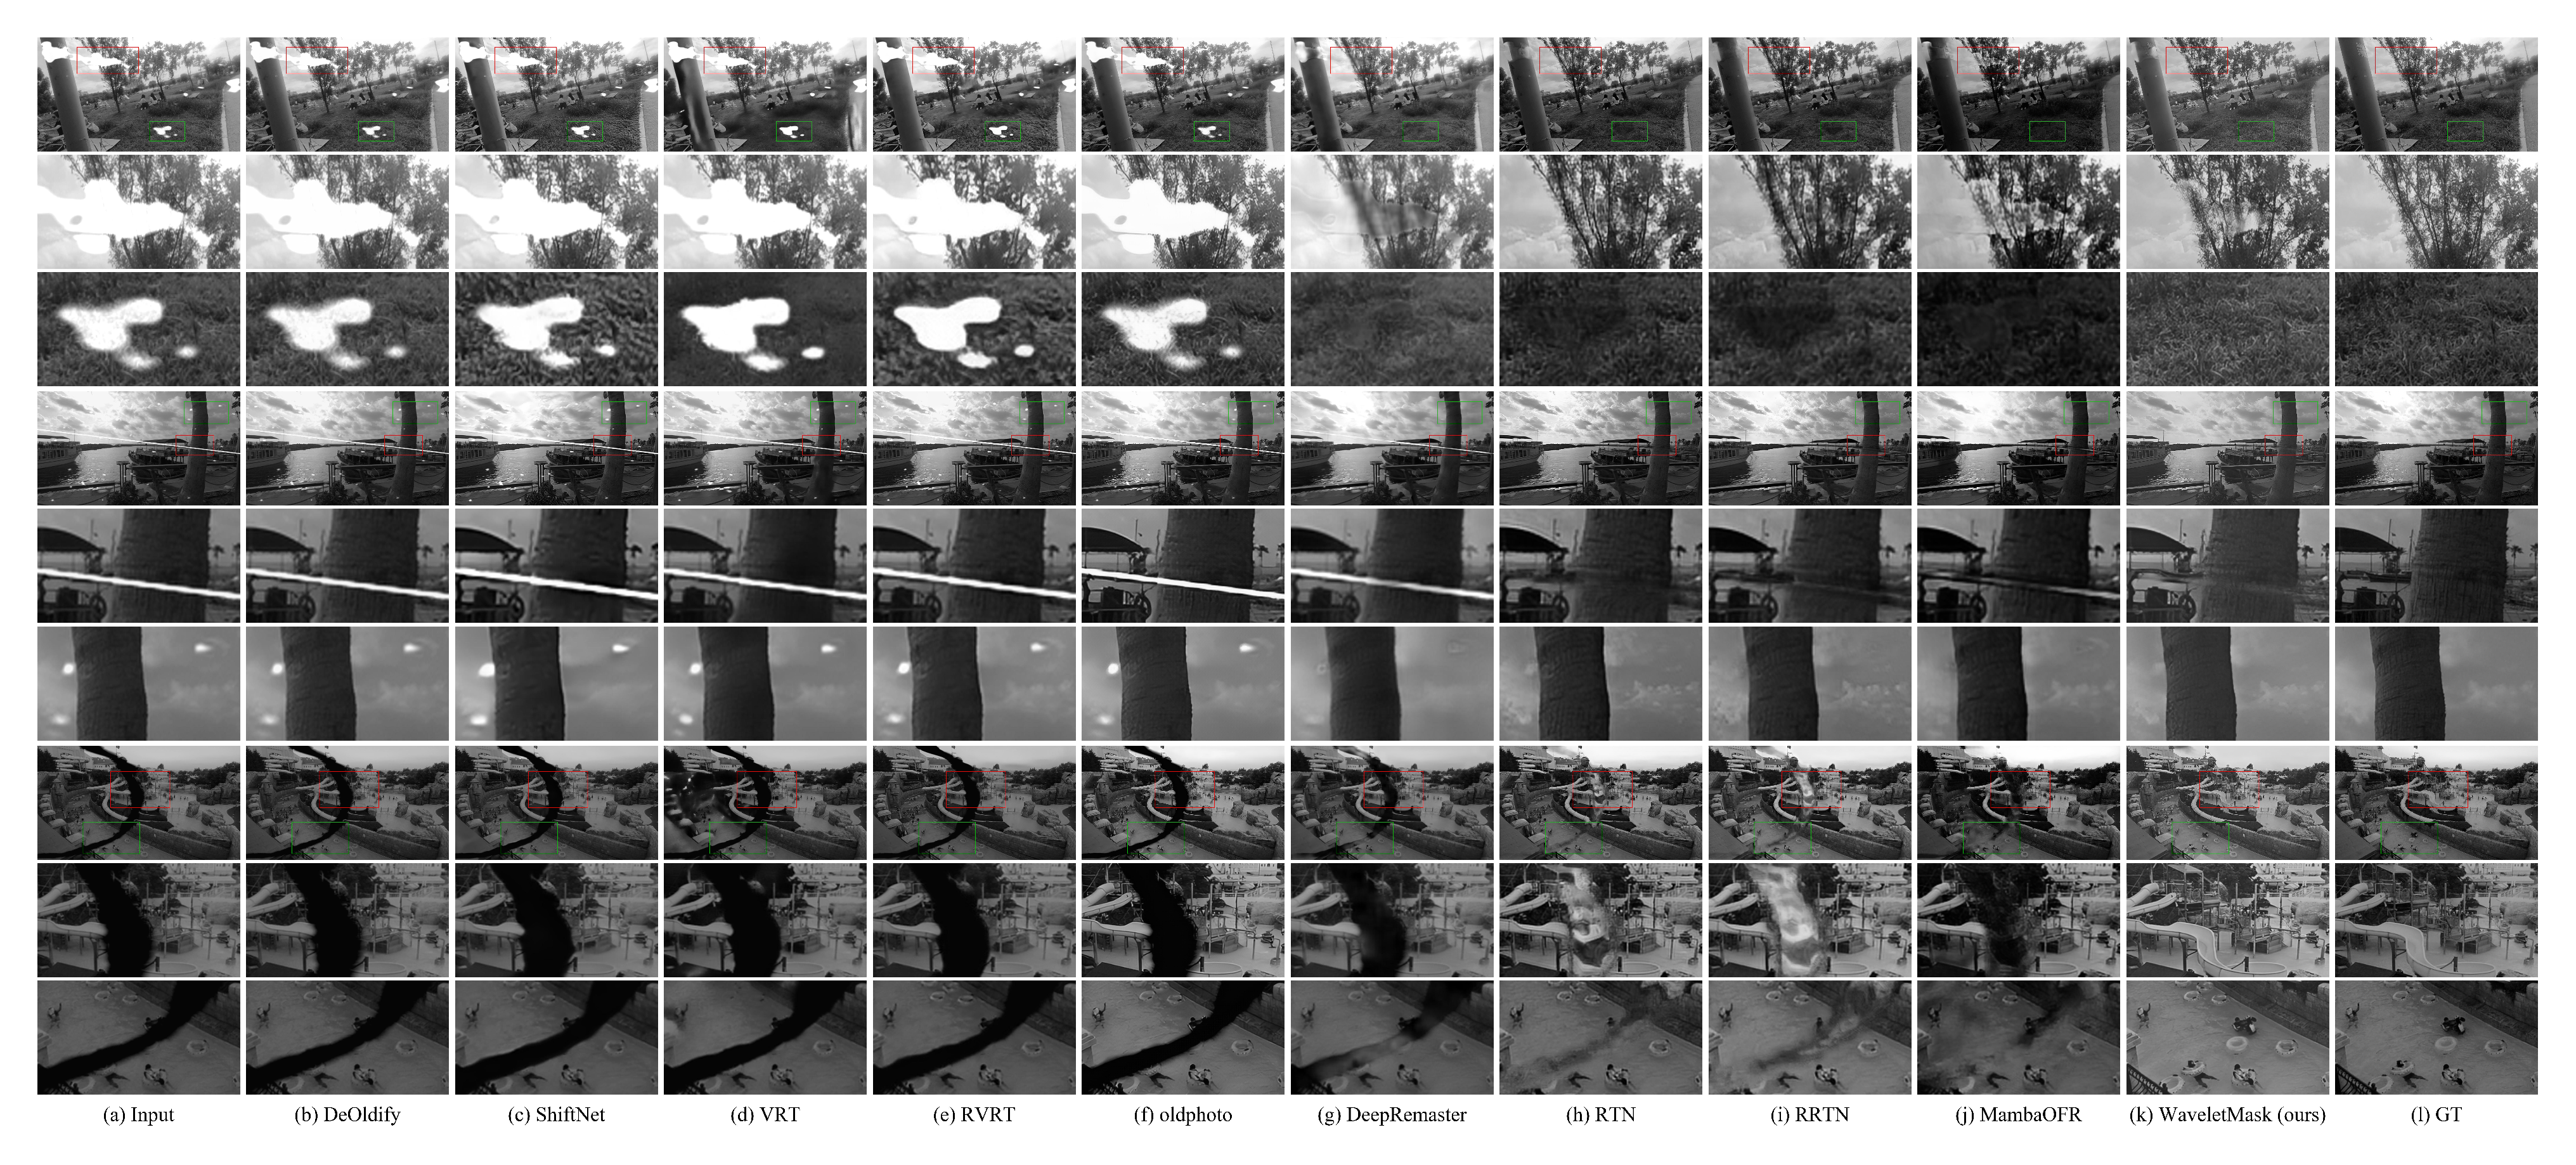
\includegraphics[width=\textwidth]{figures/Figure5.pdf}
\caption{Qualitative comparison on synthetic old-film degradation from the SRWOV/REDS synthetic test setting. Columns: (a) input, (b) DeOldify, (c) ShiftNet, (d) VRT, (e) RVRT, (f) OldPhoto, (g) DeepRemaster, (h) RTN, (i) RRTN, (j) MambaOFR, (k) WaveletMask, and (l) ground truth (GT). ROI crops highlight selected damage regions.\label{fig:sota_synthetic}}
\end{figure}

\begin{figure}[t]
\centering
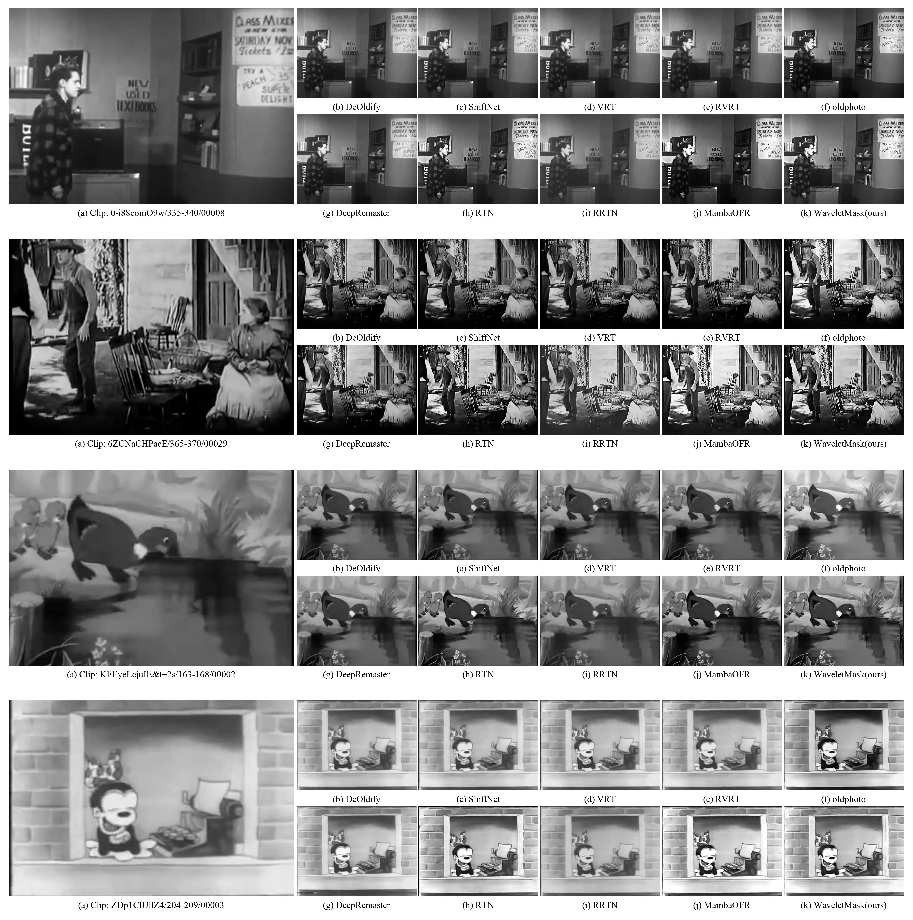
\includegraphics[width=\textwidth]{figures/Figure6.pdf}
\caption{Qualitative comparison on SRWOV real-world archival clips without paired ground truth. Each row compares one input clip/ROI with outputs from (b) DeOldify, (c) ShiftNet, (d) VRT, (e) RVRT, (f) OldPhoto, (g) DeepRemaster, (h) RTN, (i) RRTN, (j) MambaOFR, and (k) WaveletMask. Full-reference scores are unavailable for this split.\label{fig:sota_realworld}}
\end{figure}

Figure~\ref{fig:sota_synthetic} shows representative synthetic examples, where WaveletMask removes scratch and dust residuals more cleanly than the RTN output in the highlighted ROIs. Figure~\ref{fig:sota_realworld} shows the same tendency on archival clips, with cleaner local damage removal and more stable brightness restoration while preserving scene appearance. Spatial error-map analysis confirms that the gains are concentrated in damaged regions (Supplementary Figure~S5). The overall improvement raises the question of whether the gain is uniform across degradation types, which is analyzed in Appendix~\ref{subsec:artifact_breakdown}.

\subsection{Ablation Study}\label{subsec:ablation}

The ablation study is organized around four questions:
\begin{itemize}
\item \textbf{Q1 (Branch effectiveness).} Do LHFM and GFM each improve over the RTN pixel-domain gate, and are the two branches complementary?
\item \textbf{Q2 (Fusion rule).} Is parameter-free branch-level maximum fusion preferable to learned pixel-wise fusion?
\item \textbf{Q3 (Wavelet family).} How sensitive is the gate to the wavelet basis and the number of decomposition levels?
\item \textbf{Q4 (Robustness).} Do the gains persist across artifact types, motion and occlusion levels, and unseen content (Appendix~\ref{app:robustness})?
\end{itemize}

Questions Q1--Q3 are addressed by the three panels of Table~\ref{tab:ablation_core}, while Q4 is examined in Appendix~\ref{app:robustness}. To isolate the contribution of the wavelet-domain branches and the key design choices, Table~\ref{tab:ablation_core} groups three sets of contrasts under the same RTN backbone and training recipe: (a) the detection-branch components (RTN, +LHFM only, +GFM only, and the full WaveletMask variant with branch-level maximum fusion as defined in Equation~\eqref{eq:wavelet_mask}); (b) the key fusion-strategy contrasts between the parameter-free maximum rule and learned CNN fusion; and (c) the key wavelet-family contrasts around the single-level Haar default. The RTN, WaveletMask, and panel (c) rows are measured under the primary Y-channel re-test, whereas the +LHFM only, +GFM only, and learned-fusion rows come from an earlier identical-recipe evaluation run with a slightly different LPIPS/DISTS configuration; the cross-run drift is below 0.002 on these two metrics and does not affect the within-panel ranking.

\begin{table}[H]
\caption{Ablation study on SRWOV synthetic data: panel (a) compares the detection-branch components, panel (b) the proposed branch-level maximum rule against representative learned-fusion variants, and panel (c) representative wavelet families. All variants share the same RTN backbone and training recipe. Within panel (a), best results are in \textcolor{red}{red} and second-best results in \textcolor{blue}{blue}.\label{tab:ablation_core}}
\footnotesize
\begin{tabularx}{\textwidth}{lCCCC}
\toprule
\textbf{Variant} & \textbf{PSNR$\uparrow$} & \textbf{SSIM$\uparrow$} & \textbf{LPIPS$\downarrow$} & \textbf{DISTS$\downarrow$} \\
\midrule
\multicolumn{5}{l}{\textit{(a) Detection-branch components}} \\
RTN     & 26.1648 & 0.8923 & 0.1023 & 0.0946 \\
+LHFM only       & \textcolor{blue}{26.3778} & \textcolor{blue}{0.8966} & \textcolor{blue}{0.0914} & \textcolor{red}{0.0790} \\
+GFM only        & 26.1024 & \textcolor{red}{0.8980} & 0.0969 & 0.0916 \\
\textbf{WaveletMask (max fusion)} & \textcolor{red}{26.6125} & 0.8954 & \textcolor{red}{0.0886} & \textcolor{blue}{0.0827} \\
\midrule
\multicolumn{5}{l}{\textit{(b) Fusion strategy (key contrasts)}} \\
Branch-level maximum (proposed) & 26.6125 & 0.8954 & 0.0886 & 0.0827 \\
Gated CNN fusion & 26.3515 & 0.8966 & 0.0869 & 0.0842 \\
Max + pixel-wise CNN fusion & 24.9827 & 0.8896 & 0.1068 & 0.0867 \\
\midrule
\multicolumn{5}{l}{\textit{(c) Wavelet family (key contrasts)}} \\
Haar, single level (proposed) & 26.6125 & 0.8954 & 0.0886 & 0.0827 \\
Haar, two levels & 26.5175 & 0.9011 & 0.0847 & 0.0760 \\
DTCWT (dual-tree complex) & 26.4506 & 0.8992 & 0.0862 & 0.0780 \\
Daubechies-2 & 17.9208 & 0.6473 & 0.4136 & 0.3154 \\
\bottomrule
\end{tabularx}
\normalsize
\end{table}

Panel (a) of Table~\ref{tab:ablation_core} shows that LHFM alone improves PSNR by $+0.21$~dB over the RTN and yields the lowest DISTS, confirming the value of high-frequency local cues. GFM alone slightly reduces PSNR ($-0.06$~dB) but achieves the best SSIM, indicating stronger structural consistency. The full WaveletMask model reaches 26.61~dB, a $+0.45$~dB gain over RTN and the best LPIPS among the four variants. This is because LHFM targets local scratches and dust, whereas GFM stabilizes low-frequency temporal brightness variation, so their fusion provides complementary guidance. The combined improvement is larger than the arithmetic sum of the individual PSNR changes ($+0.21-0.06=+0.15$~dB), which further supports the complementarity of the two branches.

Panel (b) condenses the fusion-strategy finding: every learned-fusion variant underperforms its direct counterpart in PSNR under the tested recipe (within the fusion-ablation evaluation run, the gated CNN variant trails the maximum rule by 0.25~dB and the max+CNN variant by 1.62~dB), because the compact CNN must fuse heterogeneous sparse cues only through the final restoration loss, making optimization less stable than the parameter-free maximum rule. The gated variant does attain slightly better SSIM and LPIPS than the maximum rule, but it remains behind on PSNR and DISTS, whereas the max+CNN variant is inferior on all four metrics; the parameter-free rule therefore remains the preferred default for the fidelity-oriented design goal. Panel (c) condenses the wavelet-family finding: single-level Haar is the most stable PSNR-oriented default, Haar two-level and DTCWT remain competitive with small PSNR costs and partial perceptual gains, and longer-support wavelets fail catastrophically because filter lengths exceeding two require boundary padding in the wavelet analysis, which introduces border artifacts into the half-resolution sub-band maps processed by the detector heads. The complete fusion comparison, the full wavelet-family and stronger-fusion sweeps, and a cross-domain frequency-operator diagnostic that situates Haar among Sobel/Laplacian, Gaussian-pyramid, Fourier-temporal, and learned shallow alternatives are reported in Appendix~\ref{app:complexity_details} (Tables~\ref{tab:fusion_comparison} and~\ref{tab:followup_ablations}) and Appendix~\ref{app:diagnostics} (Table~\ref{tab:cross_domain_frequency_ablation}).

Figure~\ref{fig:ablation} visually supports the same trend: LHFM mainly removes local scratches, GFM mainly stabilizes frame-level brightness, and the full model combines both effects. Beyond these end-to-end ablations, four detector diagnostic probes confirm that the two branches are complementary rather than redundant and that the fused mask aligns with residual-proxy regions (Appendix~\ref{app:diagnostics}).

\begin{figure}[H]
\centering
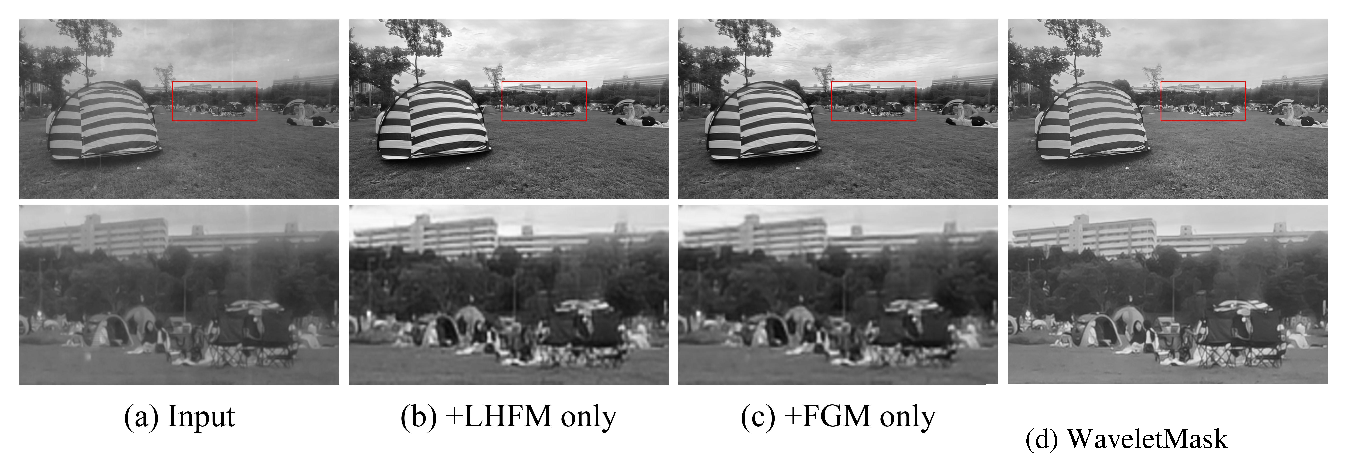
\includegraphics[width=\textwidth]{figures/Figure7.pdf}
\caption{Ablation visual comparison on selected synthetic old-film examples. Columns: (a) degraded input, (b) +LHFM only, (c) +GFM only, and (d) WaveletMask. ROIs mark local damage regions.\label{fig:ablation}}
\end{figure}

\subsection{Computational Complexity}\label{subsec:complexity}

Table~\ref{tab:complexity} summarizes parameters, floating point operations (FLOPs), and runtime cost. We report these figures to make the cost of the proposed detector explicit rather than to claim minimum latency. All rows are measured by us under one unified protocol on the same device, so the comparison is consistent across methods; the deployment-relevant quantity is the overhead that the proposed gate adds to its host network.

\begin{table}[H]
\caption{Computational cost measured by us under one unified protocol on a single NVIDIA L40 GPU in FP32 (batch size 1, seven-frame $256\times256$ clips, three warm-up and ten timed runs). Parameters and FLOPs cover the full executable forward pass on a $1\times7\times3\times256\times256$ input and include the RAFT flow estimator for the flow-based methods (RTN, RRTN, MambaOFR, WaveletMask); DeepRemaster uses no flow estimator. Latency is reported per seven-frame clip. The measurement protocol and additional batch/resolution settings are detailed in Appendix~\ref{app:complexity_details}.\label{tab:complexity}\label{tab:runtime_benchmark}}
\footnotesize
\begin{tabularx}{\textwidth}{lCCCCC}
\toprule
\textbf{Method} & \textbf{Params (M)} & \textbf{FLOPs (G)} & \textbf{Latency (ms/clip)$\downarrow$} & \textbf{Throughput (fps)$\uparrow$} & \textbf{Peak Mem. (GB)$\downarrow$} \\
\midrule
DeepRemaster~\cite{iizuka2019deepremaster}  & 9.8781 & 914.0  & 17.9  & 391.6 & 0.35 \\
RTN~\cite{rtn2022}                          & 5.7351 & 2184.7 & 169.5 & 41.3  & 0.24 \\
RRTN~\cite{rrtn2024}                        & 7.0503 & 2782.2 & 298.4 & 23.5  & 0.75 \\
MambaOFR~\cite{mao2025mambaofr}             & 8.2984 & 2832.8 & 404.8 & 17.3  & 0.60 \\
\midrule
WaveletMask                                 & 5.7360 & 2184.9 & 171.4 & 40.8  & 0.24 \\
\bottomrule
\end{tabularx}
\normalsize
\end{table}

The proposed detector adds 898 learnable parameters and 0.1494G FLOPs to the RTN, with nearly identical latency (171.4 vs.\ 169.5~ms per clip) and identical peak memory. At $1280\times720$, batch-size-1 inference takes about 5.4~s per seven-frame clip with 9.9~GB peak memory for both models, so WaveletMask inherits the cost profile of its backbone and is not yet real-time at high resolution in FP32. The full measurement protocol, additional batch and resolution settings, and the per-module parameter breakdown of the detection pathway are provided in Appendix~\ref{app:complexity_details} (Table~\ref{tab:module_overhead}).


%%%%%%%%%%%%%%%%%%%%%%%%%%%%%%%%%%%%%%%%%%
\section{Discussion}\label{sec:discussion}

\subsection{Why the Wavelet-Domain Cues Help}\label{subsec:fusion_insight}\label{subsec:freq_complement}\label{subsec:wavelet_choice}

The revised evidence supports a focused interpretation of the main result. Under the unified re-training protocol, WaveletMask improves the RTN on the synthetic benchmark (Table~\ref{tab:ablation_core}), so the most stable conclusion is not that every metric moves in the same direction, but that wavelet-domain priors improve the overall trade-off between structural repair and perceptual plausibility, which supports the proposed mask as an auxiliary restoration cue rather than a dataset-specific optimization artifact. Consistent with this, the DAVIS experiment (Table~\ref{tab:davis_cross_content}) changes the underlying scenes while keeping the degradation pipeline fixed, and the gain over the RTN persists, indicating that the cue is not tied to one video category, camera motion pattern, or clip identity, although cross-degradation generalization remains open.

\textbf{Why parameter-free maximum fusion is preferred.}
The fusion ablation in Table~\ref{tab:fusion_comparison} is best stated directly: among the tested strategies, the parameter-free branch-level maximum rule is the most reliable choice for the current learned-fusion design, the $b=+5$ spatial-prior initialization, the 200K-iteration training budget, and the reconstruction-only supervision, which is an architecture- and training-specific finding rather than a general verdict against learned fusion. The likely reason is the heterogeneity of the two inputs: LHFM is sparse and highly localized, whereas GFM is broader and tied to low-frequency photometric change, so a learned convex mixture can attenuate a sparse but informative response when the other input is weak but spatially widespread. The branch-level maximum rule avoids this mismatch by preserving the stronger cue at each location, which is especially useful when the two branches encode different temporal assumptions rather than two noisy estimates of the same quantity.

The same picture also clarifies why the flow-compensated (FC) variant does not surpass the uncompensated setting: compensating before mask formation can blur the inter-frame deviations that LHFM exploits and may inject optical-flow errors around occlusion boundaries, and because RTN-style propagation already performs temporal alignment downstream~\cite{rtn2022,rrtn2024}, the uncompensated mask preserves old-film defect contrast better, consistent with the motion-binned analysis in which the improvement is largest in the high-motion and high-occlusion terciles (Table~\ref{tab:motion_binning}).

\textbf{What the frequency-domain cues add.}
The frequency-domain design is most interpretable when LHFM and GFM are read as modeling two different classes of temporal irregularity. LHFM targets thin, spatially localized, high-frequency defects such as dust and narrow scratches: Haar detail sub-bands retain these abrupt local changes while suppressing much of the low-frequency scene content, so wavelet-domain inter-frame differences become more sensitive to defect-like perturbations than raw pixel differences, which matches the LHFM gains in Table~\ref{tab:ablation_core} and recent \textit{Applied Sciences} findings that frequency-domain representations are particularly effective for structured degradations~\cite{kim2025hybrid,park2025spatialfrequency}. GFM instead encodes gradual low-frequency photometric instability; its broader response profile is expected because flicker is a frame-level or region-level brightness inconsistency rather than a point artifact, which also explains why GFM tends to help SSIM more than PSNR in Table~\ref{tab:ablation_core}.

Two diagnostics reinforce this reading. The complementarity probe (Table~\ref{tab:cue_complementarity}) shows that the original RTN spatial indicator, LHFM, and GFM do not activate on identical regions and that the two wavelet branches are nearly disjoint in their top-response areas, precisely the regime in which branch-wise preservation is more appropriate than premature averaging. The residual-proxy probe (Table~\ref{tab:mask_interpretability}) shows strong alignment of GFM and the max-fused mask with the low-frequency proxy, while the weaker alignment of LHFM indicates that it functions as a gating prior for recurrent restoration rather than as a surrogate for supervised scratch or dust segmentation. This also positions WaveletMask relative to learned all-in-one restoration models such as AirNet, PromptIR, and MambaOFR~\cite{li2022airnet,potlapalli2023promptir,mao2025mambaofr}: instead of learning degradation representations at global, prompt, or state-space levels, WaveletMask injects a dense, hand-structured temporal cue into an RTN-style recurrent gate, trading generality for low overhead and interpretability.

\textbf{Wavelet family choice.}
Finally, the wavelet-family sweep (Table~\ref{tab:followup_ablations}) indicates that the benefit does not come from adding an arbitrary transform. Single-level Haar remains the most stable default under the current training budget, two-level Haar improves several perceptual metrics at a small PSNR cost, more oscillatory families such as db2 and sym2 are less stable in this lightweight setting, and DTCWT remains competitive but does not surpass Haar; for sparse old-film defects, sharp spatial localization is more valuable than a richer but less localized basis, and Haar's fixed $2\times2$, parameter-free filters match this goal. The cross-domain diagnostic (Table~\ref{tab:cross_domain_frequency_ablation}) narrows the claim: Fourier temporal responses and proxy-supervised shallow filters can align more strongly with residual-proxy labels, so Haar is the most stable \emph{tested} wavelet for end-to-end restoration gating rather than a universally optimal frequency detector. This is consistent with wavelet-based restoration work showing that decompositions can enlarge effective receptive fields~\cite{liu2018mwcnn} and that complex-valued transforms offer richer directional selectivity and approximate shift invariance~\cite{selesnick2005dual}, while for mask construction in old film restoration the simpler Haar basis already captures the defect statistics that matter most under the current recipe.

\subsection{Transferability, Boundary Conditions, and Evaluation Scope}\label{subsec:transferability}

Two challenging cases are best understood as boundary conditions rather than contradictions of the method. First, persistent fixed scratches are difficult for LHFM by construction. The detector compares short-term differences and is most sensitive to transient, non-stationary defects; if a scratch remains in nearly the same image-plane position for three or more frames, the geometric-mean difference is attenuated and the response is strongly reduced (Table~\ref{tab:persistent_scratch_probe}). Drifting scratches are less problematic because they continue to produce inter-frame inconsistency. The relevant conclusion is therefore not that LHFM fails on scratches in general, but that it faces challenges when the degradation becomes temporally stationary.

Second, GFM assumes gradual photometric evolution. Scene cuts and abrupt exposure flashes violate this assumption, so elevated GFM responses around such events are expected (Table~\ref{tab:gfm_failure_probe}). The luminance-difference guard already shows that most of this false activation can be suppressed without changing the backbone. Scene cuts should therefore be treated as a boundary condition of the current cue definition, not as evidence against low-frequency flicker modeling itself.

The no-reference evaluation on real footage should be interpreted with the same care. BRISQUE and NIQE are both natural-scene-statistics measures, but they are built on different priors: BRISQUE is opinion-aware and operates in the spatial domain~\cite{mittal2012brisque}, whereas NIQE is opinion-unaware and measures deviation from pristine-image statistics without distortion-specific training~\cite{mittal2013niqe}. CLIPIQA+, in turn, derives its preference from CLIP-based visual-language priors and is therefore more sensitive to semantic and perceptual plausibility~\cite{wang2023clipiqa}. Old-film restoration often changes grain, contrast, local sharpness, and semantic realism at the same time, so disagreement among BRISQUE, NIQE, and CLIPIQA+ is not only possible but expected. Recent \textit{Applied Sciences} work on no-reference assessment likewise emphasizes the limited universality of individual NR metrics and the value of combining complementary indicators instead of relying on a single score~\cite{rubel2022combinednr}. For this reason, the no-reference metrics are interpreted jointly with the qualitative comparisons rather than individually.

The scope of the comparison protocol should also be stated explicitly. All ten methods, including WaveletMask, were re-trained and re-evaluated under one unified benchmark pipeline (Table~\ref{tab:literature_context}), which supports a direct cross-method ranking on the synthetic split. To isolate the proposed gate from training confounds, RTN and WaveletMask were additionally compared under a strictly identical paired protocol (Appendix~\ref{app:stats}, Table~\ref{tab:same_protocol_main}). The two views are complementary: the controlled paired comparison remains the primary evidence for the proposed gate, while the unified benchmark situates the magnitude of the gains within the old film restoration landscape.

\subsection{Limitations and Future Work}\label{subsec:limitations}

Despite the encouraging evidence, several limitations define the current scope. First, all full-reference experiments rely on the SRWOV degradation pipeline. The DAVIS study confirms cross-content transfer, but transfer to independently synthesized degradations or real paired archival benchmarks remains open. Second, the present multi-seed analysis is stronger than a single-run report yet still modest; a larger five-seed or ten-seed study would provide tighter uncertainty estimates. Third, the mask is computed without explicit scene-cut awareness and without explicit mask supervision, so it may fail to detect temporally stationary damage and may produce false activation around abrupt editing events; in addition, clip-boundary frames lack bilateral temporal neighbors and are assigned zero wavelet masks, so the first and last frames of each clip currently receive no wavelet-domain degradation cue. Fourth, while the motion- and occlusion-binned analysis in Table~\ref{tab:motion_binning} shows that ordinary motion does not erode the restoration gain on the present benchmark, that evidence is camera-motion dominated and tercile-grained; object-dominant motion, extreme displacements, and absolute motion thresholds remain to be characterized. Fifth, the cross-domain diagnostic in Table~\ref{tab:cross_domain_frequency_ablation} shows that Fourier-temporal and proxy-supervised operators can align more strongly with residual proxies than frozen Haar responses, and these alternatives have not yet been retrained end-to-end inside the gating pipeline; the present evidence therefore supports Haar as the most stable tested wavelet choice rather than the optimal frequency operator. Finally, very large missing regions or long-term severe deterioration prove difficult for the current restoration-only formulation, because the problem gradually shifts from defect suppression to content completion.

These limitations suggest several concrete next steps. A first direction is event-aware gating, including scene-cut and flash detectors for GFM and persistence-aware detectors for stationary scratches. A second direction is to revisit learned fusion with stronger supervision, uncertainty calibration, and longer schedules, since the current max rule likely benefits from its robustness to scale mismatch more than from greater expressive power. A third direction is to couple restoration with explicit completion modules when film loss becomes spatially extensive; recent \textit{Applied Sciences} work on unified inpainting and colorization provides a useful template for this scenario~\cite{yeo2025integration}. Finally, broader validation on real archival collections and a larger public release of per-run evidence would strengthen both the empirical claims and the reproducibility value of the work.

Overall, the results support a balanced claim: WaveletMask is a lightweight and interpretable improvement for RTN-style old film restoration when degradations remain temporally informative, while persistent structural damage, abrupt temporal discontinuities, and large missing regions define the main frontier for future development.


%%%%%%%%%%%%%%%%%%%%%%%%%%%%%%%%%%%%%%%%%%
\section{Conclusions}\label{sec:conclusions}

In this paper, we propose WaveletMask to improve recurrent old film restoration by replacing the raw pixel-domain gate cue with a wavelet-domain gate that captures local high-frequency damage responses and global flicker responses. On the unified SRWOV re-training benchmark, WaveletMask attains the best PSNR among ten uniformly re-trained methods while adding only 898 detector parameters and remaining competitive on the perceptual metrics, and a strict paired comparison against the RTN confirms a statistically significant clip-level PSNR improvement. Additional robustness experiments across three random seeds and artifact-stratified analyses further show that the wavelet-domain gate is particularly effective for scratch- and flicker-related degradations. Beyond full-reference evaluation, the method also shows practical value on real archival clips: WaveletMask is the only method placing within the top two on all three no-reference metrics (narrowly so on CLIPIQA+), and the qualitative comparisons show cleaner scratch and flicker removal with better-preserved film texture and temporal stability. Taken together, these findings indicate that WaveletMask provides a lightweight and effective degradation-aware gating strategy for old film restoration. Because the wavelet-domain gate adds only 898 detector parameters on top of an existing recurrent backbone, it can be integrated as a drop-in gating cue into current restoration pipelines, making it practical for large-scale archival-film and legacy-video remastering where per-clip overhead matters.

These gains nonetheless come with clear boundary conditions: persistent image-plane-fixed scratches, abrupt temporal discontinuities such as scene cuts, and spatially extensive film losses remain challenging for the current restoration-only formulation (Section~\ref{subsec:limitations}). Future work can further improve persistent scratch handling and replace the current fusion design with learned fusion under explicit supervision. It is also important to evaluate the method on more diverse real-world archival datasets to strengthen cross-degradation generalization and robustness in challenging restoration scenarios.


%%%%%%%%%%%%%%%%%%%%%%%%%%%%%%%%%%%%%%%%%%
\vspace{6pt} 

%%%%%%%%%%%%%%%%%%%%%%%%%%%%%%%%%%%%%%%%%%
\authorcontributions{Conceptualization, F.C. and Y.D.; methodology, F.C.; software, F.C.; validation, F.C. and Q.Z.; formal analysis, F.C.; investigation, F.C.; resources, Y.D.; data curation, F.C.; writing---original draft preparation, F.C.; writing---review and editing, C.-A.X. and Y.D.; visualization, F.C.; supervision, Y.D.; project administration, Y.D. All authors have read and agreed to the published version of the manuscript.}

\funding{This research received no external funding.}

\institutionalreview{The study was conducted in accordance with the Declaration of Helsinki. All algorithmic experiments in this work were conducted on publicly available video datasets for old-film restoration evaluation. The expert subjective image-quality evaluation mentioned in the manuscript was an internal visual-quality scoring of restored images by internal expert raters; it did not recruit external human subjects, collect human biological samples, record identifiable personal or private information, or involve any intervention on the human body. In accordance with Article 2 of the \emph{Measures for Scientific and Technological Ethics Review (Trial)} (Guo Ke Fa Jian [2023] No. 167; jointly issued by the Ministry of Science and Technology and nine other Chinese authorities), this work does not fall within the scope requiring mandatory ethics review, and no ethics approval or exemption document is required.}

\informedconsent{Not applicable. No external human subjects were recruited, and the internal visual-quality scoring did not collect identifiable personal or private information.}

\dataavailability{The REDS dataset used for training is publicly available at \url{https://seungjunnah.github.io/Datasets/reds.html}. The SRWOV benchmark used for evaluation is publicly available at \url{https://github.com/MaoAYD/MambaOFR}. The synthetic degradation protocol follows the publicly described RTN/SRWOV settings. Supplementary Tables S1--S2 and Supplementary Figures S1--S6 are provided as a separate supplementary package. The code, training and evaluation configurations, same-protocol metric summaries, paired seed-2021 clip-level statistics, diagnostic scripts, and runtime-benchmark artifacts are being prepared for public release at \url{https://github.com/wscffaa/WaveletMask}; until the tagged release is posted, they are available from the corresponding author upon reasonable request. Trained model weights are not included in the public package because of file size; they will be posted with the repository release or provided by the corresponding author subject to institutional repository approval and third-party dataset license checks.}

\acknowledgments{The authors thank the developers of RTN for releasing their code and pretrained models.}

\conflictsofinterest{The authors declare no conflicts of interest.}

%%%%%%%%%%%%%%%%%%%%%%%%%%%%%%%%%%%%%%%%%%
\supplementary{The following supporting information can be downloaded as a separate supplementary package mirrored in the manuscript source files: Figure S1: complete persistent-scratch diagnostic examples; Figure S2: complete residual-proxy overlap examples; Figure S3: complete cue-complementarity examples; Figure S4: expert-level subjective evaluation results ((a) overall preference distribution; (b) rank-1 counts across three perceptual dimensions); Figure S5: error-map comparison between the RTN and WaveletMask on selected SRWOV synthetic frames; Figure S6: visualization for the wavelet-mask probes; Table S1: overall preference in the internal expert-level subjective evaluation (34 internal expert raters $\times$ 14 clips); Table S2: rank-1 counts by perceptual dimension.}

%%%%%%%%%%%%%%%%%%%%%%%%%%%%%%%%%%%%%%%%%%
\abbreviations{Abbreviations}{
The following abbreviations are used in this manuscript:
\\

\noindent 
\begin{tabular}{@{}ll}
OFR & Old Film Restoration\\
DWT & Discrete Wavelet Transform\\
LHFM & Local High-Frequency Mask Module\\
GFM & Global Flicker Mask Module\\
HF & High Frequency\\
LF & Low Frequency\\
RTN & Recurrent Transformer Network\\
RRTN & Recursive Recurrent Transformer Network\\
SRWOV & Synthetic and Real-World Old Video (benchmark)\\
REDS & REalistic and Dynamic Scenes dataset\\
RAFT & Recurrent All-Pairs Field Transforms\\
ROI & Region of Interest\\
GT & Ground Truth\\
PSNR & Peak Signal-to-Noise Ratio\\
SSIM & Structural Similarity Index Measure\\
LPIPS & Learned Perceptual Image Patch Similarity\\
DISTS & Deep Image Structure and Texture Similarity\\
NIQE & Natural Image Quality Evaluator\\
BRISQUE & Blind/Referenceless Image Spatial Quality Evaluator\\
CLIPIQA+ & CLIP-based Image Quality Assessment (prompt-tuned variant)\\
CLIP & Contrastive Language--Image Pre-training\\
CNN & Convolutional Neural Network\\
RNN & Recurrent Neural Network\\
GAN & Generative Adversarial Network\\
VGG & Visual Geometry Group network\\
GPU & Graphics Processing Unit\\
FLOPs & Floating Point Operations\\
MAE & Mean Absolute Error\\
RGB & Red--Green--Blue color space\\
BT.601 & ITU-R BT.601 luminance transform\\
LL/LH/HL/HH & Wavelet sub-bands (Low--Low / Low--High / High--Low / High--High)
\end{tabular}
}

%%%%%%%%%%%%%%%%%%%%%%%%%%%%%%%%%%%%%%%%%%
\appendixtitles{yes}
\appendixstart
\appendix
\section{Statistical Reliability of the Paired Comparison}\label{app:stats}

Under the strict paired protocol, RTN and WaveletMask are trained and evaluated with the same data, degradation pipeline, implementation, and metric scripts, which isolates the contribution of the proposed wavelet-domain gate from confounding training differences. Table~\ref{tab:same_protocol_main} reports this primary seed-2021 comparison together with its clip-level paired statistics: relative to the RTN, WaveletMask improves PSNR by $+0.45$~dB and also improves SSIM, LPIPS, and DISTS, and all four paired clip-level gains are statistically significant under two-sided permutation tests. This controlled comparison complements the unified re-training benchmark over all ten methods in Section~\ref{subsec:sota_quant} (Table~\ref{tab:literature_context}).

\begin{table}[t]
\caption{Paired controlled comparison on the SRWOV synthetic benchmark (seed 2021, Y-channel protocol, 30 clips). RTN and WaveletMask share the same data, degradation pipeline, implementation, and metric scripts, so this strict paired comparison is the controlled evidence for the proposed gate. The paired improvement reports WaveletMask minus RTN for PSNR/SSIM and RTN minus WaveletMask for LPIPS/DISTS (positive favors WaveletMask); confidence intervals use clip-level bootstrap resampling and $p$-values use a two-sided paired permutation test. The WaveletMask paired-protocol PSNR (26.6125~dB) differs slightly from the unified-benchmark value in Table~\ref{tab:literature_context} (26.6017~dB) because the two protocols use different training checkpoints and metric configurations. Best values in each row are in \textcolor{red}{red}.\label{tab:same_protocol_main}\label{tab:paired_seed2021_stats}}
\footnotesize
\begin{tabularx}{\textwidth}{lCCCC}
\toprule
\textbf{Metric} & \textbf{RTN} & \textbf{WaveletMask} & \textbf{Paired improvement} & \textbf{95\% CI / two-sided $p$} \\
\midrule
PSNR$\uparrow$  & 26.1648 & \textcolor{red}{26.6125} & $+0.4477$ & $[0.2955, 0.5981]$, $p=5\times10^{-5}$ \\
SSIM$\uparrow$  & 0.8923  & \textcolor{red}{0.8954}  & $+0.0031$ & $[0.0014, 0.0050]$, $p=1.5\times10^{-3}$ \\
LPIPS$\downarrow$ & 0.1023 & \textcolor{red}{0.0886} & $+0.0137$ & $[0.0108, 0.0166]$, $p=5\times10^{-5}$ \\
DISTS$\downarrow$ & 0.0946 & \textcolor{red}{0.0827} & $+0.0119$ & $[0.0103, 0.0136]$, $p=5\times10^{-5}$ \\
\bottomrule
\end{tabularx}
\normalsize
\end{table}

\begin{table}[H]
\caption{Three-seed same-protocol Y-channel re-test on the SRWOV synthetic benchmark. Values are mean$\pm$standard deviation over seeds 2021, 2022, and 2023. Best results are in \textcolor{red}{red}.\label{tab:three_seed_summary}}
\begin{tabularx}{\textwidth}{lCCCC}
\toprule
\textbf{Method} & \textbf{PSNR$\uparrow$} & \textbf{SSIM$\uparrow$} & \textbf{LPIPS$\downarrow$} & \textbf{DISTS$\downarrow$} \\
\midrule
RTN~\cite{rtn2022} & 24.5570$\pm$1.6667 & 0.8808$\pm$0.0129 & 0.1083$\pm$0.0118 & 0.0922$\pm$0.0040 \\
\textbf{WaveletMask (ours)} & \textcolor{red}{26.2183$\pm$0.3725} & \textcolor{red}{0.8983$\pm$0.0045} & \textcolor{red}{0.0879$\pm$0.0026} & \textcolor{red}{0.0831$\pm$0.0015} \\
\midrule
Mean difference & +1.6613 & +0.0175 & -0.0205 & -0.0091 \\
\bottomrule
\end{tabularx}
\end{table}

Table~\ref{tab:three_seed_summary} shows that the advantage persists across seeds and that WaveletMask is markedly more stable than the baseline: the PSNR standard deviation drops from 1.67~dB (RTN) to 0.37~dB (WaveletMask), and all four metric means improve. For transparency, the per-seed PSNR values under seeds 2021/2022/2023 are 26.1648/24.6691/22.8370~dB for the RTN and 26.6125/26.1702/25.8721~dB for WaveletMask, so WaveletMask outperforms the baseline under every individual seed rather than only on average. The paired controlled comparison in Table~\ref{tab:same_protocol_main} uses seed 2021, under which the baseline attains its strongest result, making the reported $+0.45$~dB gain the most conservative of the three seeds.

\section{Robustness and Cross-Content Generalization}\label{app:robustness}

This appendix examines whether the same-protocol gain reported in Section~\ref{subsec:sota_quant} is concentrated in one degradation pattern, degrades under stronger motion or occlusion, or fails to transfer beyond REDS source content.

\subsection{Artifact-Dominant Synthetic Breakdown}\label{subsec:artifact_breakdown}

To examine whether the same-protocol gain is concentrated in one degradation pattern, we stratified the 30 SRWOV synthetic clips by paired input--ground-truth residual descriptors. The descriptors measure elongated high-residual components for scratch-like structure, compact high-residual components for dust-like spots, and low-frequency mean-shift responses for flicker-like brightness variation. This procedure gives clip-level artifact-dominant strata; it is not a pixel-level generator-label annotation. Table~\ref{tab:artifact_breakdown} aggregates the per-clip metrics from the RTN and WaveletMask logs within each stratum.

\begin{table}[H]
\caption{Artifact-dominant breakdown on the SRWOV synthetic benchmark. Clip strata are formed from paired input--ground-truth residual descriptors. The improvement columns report gains of WaveletMask over the RTN (positive favors WaveletMask); for LPIPS and DISTS, the improvement is the error reduction.\label{tab:artifact_breakdown}}
\footnotesize
\begin{tabularx}{\textwidth}{lccCCCC}
\toprule
& & & & \multicolumn{3}{c}{\textbf{Improvement over RTN}} \\
\cmidrule(lr){5-7}
\textbf{Stratum} & \textbf{Clips} & \textbf{RTN PSNR} & \textbf{WaveletMask PSNR} & \textbf{PSNR (dB)} & \textbf{SSIM} & \textbf{LPIPS / DISTS} \\
\midrule
Scratch-dominant & 5  & 27.47 & 28.11 & +0.64 & +0.0020 & +0.0110 / +0.0116 \\
Dust-dominant    & 8  & 26.10 & 26.55 & +0.45 & +0.0049 & +0.0196 / +0.0120 \\
Flicker-dominant & 6  & 23.90 & 24.37 & +0.47 & +0.0055 & +0.0176 / +0.0153 \\
Mixed residual   & 11 & 26.83 & 27.17 & +0.34 & +0.0017 & +0.0102 / +0.0109 \\
\bottomrule
\end{tabularx}
\normalsize
\end{table}

Table~\ref{tab:artifact_breakdown} shows positive PSNR, SSIM, LPIPS, and DISTS gains in all four strata. The largest PSNR gain appears in the scratch-dominant group, whereas the flicker-dominant group shows the largest SSIM and DISTS improvements. This pattern indicates that the gain is not confined to a single degradation mode within the SRWOV synthetic setting, which is consistent with the complementary roles of LHFM and GFM.

\subsection{Motion- and Occlusion-Binned Analysis}\label{subsec:motion_binning}

To quantify how camera motion, object motion, and occlusion affect both the detector and the final restoration quality, we computed RAFT-based motion descriptors on the clean ground-truth frames of the 30 fixed synthetic clips: the mean optical-flow magnitude, a camera-motion proxy (the magnitude of the per-frame median flow vector), an object-motion proxy (the mean residual flow after removing the median), and a forward--backward inconsistency occlusion ratio. Clips were then stratified into motion and occlusion terciles, and the per-clip metrics of the same-protocol seed-2021 RTN and WaveletMask models were aggregated per bin. For the detector itself we report, per bin, the fraction of each cue's top-5\% activation that falls outside the residual proxy of Appendix~\ref{subsec:mask_interpretability} (clean-FP; lower is better).

\begin{table}[t]
\caption{Motion- and occlusion-binned analysis on the 30 fixed synthetic clips. Motion and occlusion descriptors are RAFT statistics on clean ground-truth frames, and bins are clip terciles rather than absolute thresholds. The improvement columns report gains of WaveletMask over the RTN (positive is better for all four metrics). Clean-FP is the fraction of each detector cue's top-5\% activation outside the residual proxy (lower is better); the max-fused mask follows the GFM column because the GFM response dominates the fused scale.\label{tab:motion_binning}}
\footnotesize
\begin{tabularx}{\textwidth}{llCCCCCCCC}
\toprule
& & & & & \multicolumn{4}{c}{\textbf{Improvement over RTN}} & \\
\cmidrule(lr){6-9}
\textbf{Group} & \textbf{Bin} & \textbf{Clips} & \textbf{Motion} & \textbf{Occl.} & \textbf{PSNR (dB)} & \textbf{SSIM} & \textbf{LPIPS} & \textbf{DISTS} & \textbf{LHFM / GFM clean-FP} \\
\midrule
Motion & Low    & 10 & 0.77 & 0.009 & +0.085 & +0.0009 & +0.0115 & +0.0127 & 0.646 / 0.440 \\
Motion & Medium & 10 & 1.87 & 0.027 & +0.477 & +0.0036 & +0.0172 & +0.0135 & 0.782 / 0.627 \\
Motion & High   & 10 & 3.90 & 0.053 & +0.769 & +0.0056 & +0.0143 & +0.0103 & 0.681 / 0.584 \\
\midrule
Occlusion & Low    & 10 & 0.85 & 0.005 & +0.186 & +0.0018 & +0.0119 & +0.0133 & 0.716 / 0.515 \\
Occlusion & Medium & 10 & 2.02 & 0.022 & +0.498 & +0.0018 & +0.0139 & +0.0113 & 0.703 / 0.541 \\
Occlusion & High   & 10 & 3.67 & 0.062 & +0.647 & +0.0065 & +0.0172 & +0.0119 & 0.690 / 0.594 \\
\bottomrule
\end{tabularx}
\normalsize
\end{table}

Table~\ref{tab:motion_binning} shows that the WaveletMask improvement does not collapse under stronger motion. The PSNR gain instead grows from +0.085~dB in the low-motion tercile to +0.477~dB (medium) and +0.769~dB (high), with a clip-level Spearman correlation of 0.58 between motion magnitude and PSNR improvement, and SSIM, LPIPS, and DISTS improve in every bin. The occlusion terciles behave consistently (+0.186/+0.498/+0.647~dB; Spearman 0.49). At the detector level, the LHFM clean-FP fraction is essentially uncorrelated with motion magnitude (Spearman $-0.04$), and the GFM fraction increases only weakly (Spearman 0.30), which matches GFM's sensitivity to global temporal change. These results indicate that, on this benchmark, motion-induced detector noise does not translate into restoration degradation; the flow-aligned recurrent propagation downstream absorbs it. These binned results also serve as the temporal-stability evidence for this work: the improvements hold and grow under stronger motion and occlusion rather than degrading, indicating that the wavelet masks do not destabilize the flow-aligned recurrent propagation. Two caveats bound this conclusion: the REDS-derived clips are camera-motion dominated (29 of 30 clips under the median-flow split), so object-dominant motion remains under-represented, and the bins are relative clip terciles on one benchmark rather than absolute motion thresholds.

\subsection{Cross-Content Generalization on DAVIS}\label{subsec:davis}

To assess whether the improvement transfers beyond REDS source content, we evaluated the same trained checkpoints on the DAVIS synthetic benchmark (50 clips, 854$\times$480) using the identical degradation pipeline but with substantially different video content (outdoor sports, animals, vehicles). To our knowledge, no publicly available paired old-film video restoration benchmark with ground truth exists beyond SRWOV/REDS-based protocols; DAVIS therefore represents the maximum feasible cross-content validation.

\begin{table}[H]
\caption{Cross-content generalization on DAVIS synthetic data (50 clips). Same degradation pipeline as REDS, different video content. Best results are in \textcolor{red}{red}. The final row reports improvement; for LPIPS and DISTS it is computed as RTN minus WaveletMask.\label{tab:davis_cross_content}}
\begin{tabularx}{\textwidth}{lCCCC}
\toprule
\textbf{Model} & \textbf{PSNR$\uparrow$} & \textbf{SSIM$\uparrow$} & \textbf{LPIPS$\downarrow$} & \textbf{DISTS$\downarrow$} \\
\midrule
RTN & 25.8417 & \textcolor{red}{0.8827} & 0.1223 & 0.1089 \\
\textbf{WaveletMask} & \textcolor{red}{25.9883} & 0.8795 & \textcolor{red}{0.1206} & \textcolor{red}{0.1048} \\
\midrule
Improvement & +0.15 & $-$0.003 & +0.002 & +0.004 \\
\bottomrule
\end{tabularx}
\end{table}

The gain persists on unseen video content, confirming cross-content transfer. Specifically, WaveletMask improves PSNR from 25.84 to 25.99~dB and also reduces LPIPS and DISTS on DAVIS, while SSIM is essentially unchanged ($-0.003$), even though DAVIS contains different subjects and motion patterns from REDS. The smaller numerical margin is consistent with DAVIS's higher motion complexity. This experiment validates cross-content transfer under the same degradation pipeline; cross-degradation transfer to independently generated artifacts or real archival footage remains a separate question.

\section{Detector Diagnostic Probes}\label{app:diagnostics}

This appendix isolates the behavior of the proposed detector under controlled probe conditions referenced from Section~\ref{subsec:ablation}: abrupt temporal transitions for GFM, persistent scratches for LHFM, residual-proxy localization for mask interpretability, and pairwise cue relations for branch complementarity. A cross-domain frequency-operator diagnostic then situates Haar among alternative frequency operators. Representative visual examples for the probes are summarized in Supplementary Figure~S6, and complete example grids are provided in Supplementary Figures~S1--S3.

\subsection{GFM Failure-Mode Probe}\label{subsec:gfm_failure_probe}

A natural concern for the GFM minimum-difference rule is that it may confuse brightness flicker with scene transitions, flashes, and abrupt illumination changes. To isolate this behavior, we generated synthetic seven-frame probe sequences from held-out REDS ground-truth clips: (1) scene cuts by replacing the second half of a clip with another clip, (2) single-frame exposure flashes, and (3) monotonic illumination ramps. We then measured the trained GFM branch response only. The false-positive rate (FPR) is computed relative to each clean source clip's 99th-percentile GFM response, and the guard column reports a simple frame-level cut detector based on mean absolute luminance differences.

\begin{table}[H]
\caption{GFM response on synthetic failure-mode probes. Activation is the mean GFM mask value on non-boundary frames. Ratio compares probe activation with the corresponding clean clip. Suppression reports the activation reduction after a simple luminance-difference cut guard, which is evaluated post hoc and is not part of the deployed WaveletMask model.\label{tab:gfm_failure_probe}}
\footnotesize
\begin{tabularx}{\textwidth}{lccCCCCC}
\toprule
\textbf{Probe} & \textbf{Clips} & \textbf{Clean act.} & \textbf{Probe act.} & \textbf{Ratio} & \textbf{FPR} & \textbf{Guarded act.} & \textbf{Suppression} \\
\midrule
Scene cut            & 12 & 0.0041 & 0.0066 & 2.35$\times$ & 0.0505 & 0.0024 & 0.6141 \\
Exposure flash       & 12 & 0.0041 & 0.0257 & 10.41$\times$ & 0.1574 & 0.0015 & 0.9470 \\
Illumination ramp    & 12 & 0.0041 & 0.0051 & 1.52$\times$ & 0.0352 & 0.0049 & 0.0247 \\
\bottomrule
\end{tabularx}
\normalsize
\end{table}

Table~\ref{tab:gfm_failure_probe} confirms the expected failure mode: the trained GFM branch responds more strongly to scene cuts and flashes than to clean clips, and the response is especially large for single-frame flashes. This is because the minimum-difference rule is sensitive to abrupt luminance discontinuities. A simple luminance-difference guard suppresses most of the scene-cut and flash activation, but it barely affects gradual illumination ramps, indicating that cut-aware GFM is a practical direction for further improvement.

\subsection{Persistent-Scratch Response Probe}\label{subsec:persistent_scratch_probe}

A complementary mechanism-level question is whether the LHFM geometric-mean criterion suppresses scratches that persist across multiple frames. To test this mechanism directly, we injected controlled synthetic scratches into clean held-out REDS clips and measured detector response at the center frame. The persistence length is $L\in\{1,2,3,5\}$ over a seven-frame clip. The \emph{fixed} mode keeps the scratch at the same image-plane location across active frames, whereas the \emph{drift} mode shifts it by two pixels per frame. Table~\ref{tab:persistent_scratch_probe} reports the raw LHFM geometric response before the learned convolutional branch and the final max-fused $m_{\mathrm{wavelet}}$ response.

\begin{table}[H]
\caption{Detector response to controlled persistent scratches. Relative response is normalized by the same mode's single-frame ($L=1$) response. Suppression is $1-\mathrm{relative}$ for the raw LHFM response.\label{tab:persistent_scratch_probe}}
\footnotesize
\begin{tabularx}{\textwidth}{lccCCCC}
\toprule
\textbf{Mode} & \textbf{$L$} & \textbf{Clips} & \textbf{Raw LHFM} & \textbf{Raw rel.} & \textbf{Raw suppression} & \textbf{$m_{\mathrm{wavelet}}$ rel.} \\
\midrule
Fixed & 1 & 12 & 0.0862 & 1.0000 & 0.0000 & 1.0000 \\
Fixed & 2 & 12 & 0.0462 & 0.5355 & 0.4645 & 0.0167 \\
Fixed & 3 & 12 & 0.0302 & 0.3498 & 0.6502 & 0.0108 \\
Fixed & 5 & 12 & 0.0302 & 0.3498 & 0.6502 & 0.0108 \\
\midrule
Drift & 1 & 12 & 0.0862 & 1.0000 & 0.0000 & 1.0000 \\
Drift & 2 & 12 & 0.0894 & 1.0364 & -0.0364 & 0.1363 \\
Drift & 3 & 12 & 0.0957 & 1.1097 & -0.1097 & 0.0419 \\
Drift & 5 & 12 & 0.0957 & 1.1097 & -0.1097 & 0.0419 \\
\bottomrule
\end{tabularx}
\normalsize
\end{table}

Table~\ref{tab:persistent_scratch_probe} confirms the expected limitation of Equation~\eqref{eq:geomean}: when the same scratch persists at the same image location, both temporal differences become smaller and the raw LHFM response drops to 0.35 of the single-frame response for $L\ge3$. This is because the geometric mean attenuates locations where both bilateral differences become small. The drift mode behaves differently because the scratch moves relative to the current frame, so the bilateral difference remains large. The final $m_{\mathrm{wavelet}}$ response is likewise strongly reduced for persistent fixed scratches, identifying this case as a failure mode of the current detector.
Complete persistent-scratch visualization grids are provided in Supplementary Figure~S1.

\subsection{Mask Interpretability and Residual-Proxy Overlap}\label{subsec:mask_interpretability}

Because the SRWOV/REDS synthetic split used in this study does not expose generator-side pixel annotations, we evaluate mask interpretability against paired input--ground-truth residual proxies rather than true artifact masks. For each sampled non-boundary frame, local proxy regions are derived from high-pass residuals, flicker proxy regions from low-frequency residual shifts, and the wavelet proxy from their union. We then measure the trained $m_{\mathrm{local}}$, $m_{\mathrm{flicker}}$, and max-fused $m_{\mathrm{wavelet}}$ masks on 30 clips with 20 sampled frames per clip. Table~\ref{tab:mask_interpretability} reports area-normalized localization statistics; the random top-5\% hit rate equals the corresponding proxy area.

\begin{table}[H]
\caption{Mask interpretability probe on SRWOV/REDS synthetic frames. Proxy regions are derived from paired input--ground-truth residuals rather than generator-side artifact annotations. AUPRC, F1, IoU, precision, and recall are computed against these residual proxies.\label{tab:mask_interpretability}}
\footnotesize
\begin{tabularx}{\textwidth}{lCCCCCCCC}
\toprule
\textbf{Mask} & \textbf{Proxy area} & \textbf{AUPRC} & \textbf{Best F1} & \textbf{Best IoU} & \textbf{Prec.} & \textbf{Rec.} & \textbf{In/Out} & \textbf{Top-5 hit} \\
\midrule
$m_{\mathrm{local}}$   & 0.0820 & 0.0552 & 0.1515 & 0.0820 & 0.0820 & 1.0000 & 0.6103 & 0.0412 \\
$m_{\mathrm{flicker}}$ & 0.2858 & 0.4888 & 0.4949 & 0.3288 & 0.4087 & 0.6271 & 3.5714 & 0.6854 \\
$m_{\mathrm{wavelet}}$ & 0.2907 & 0.4943 & 0.4996 & 0.3330 & 0.4128 & 0.6328 & 3.5638 & 0.6908 \\
\bottomrule
\end{tabularx}
\normalsize
\end{table}

Table~\ref{tab:mask_interpretability} shows that the flicker and max-fused masks are strongly concentrated in residual-proxy regions: $m_{\mathrm{wavelet}}$ reaches an AUPRC of 0.4943, an inside/outside activation ratio of 3.56, and a top-5\% hit rate of 0.6908 compared with the 0.2907 random-area baseline. The local mask behaves differently under this proxy, with a top-5\% hit rate below the random-area baseline and an inside/outside ratio below one. This suggests that the current residual proxy captures the global flicker cue more faithfully than fine local scratches or dust, even though Table~\ref{tab:ablation_core} shows that LHFM still improves restoration quality. Stronger generator-side labels or manual annotations would enable a more direct localization study.
Additional residual-proxy overlap examples are provided in Supplementary Figure~S2.

\subsection{Cue Complementarity Analysis}\label{subsec:cue_complementarity}

To test whether the wavelet cues simply reproduce the original RTN spatial indicator, we compared the trained $m_{\mathrm{local}}$ and $m_{\mathrm{flicker}}$ masks with a flow-aligned RTN spatial indicator. The spatial indicator was computed with RAFT flow and forward warping, matching the baseline mask contract. The analysis uses 12 SRWOV/REDS synthetic clips, seven frames per clip, and the five non-boundary frames in each clip. As in Appendix~\ref{subsec:mask_interpretability}, residual-proxy hits are derived from paired input--ground-truth residuals rather than generator-side artifact labels.

\begin{table}[H]
\caption{Pairwise cue relation in the flow-aligned complementarity analysis. Top-5 overlap and Jaccard are computed from each cue's top 5\% response pixels on the same frame. Low overlap indicates that two cues emphasize different spatial regions.\label{tab:cue_complementarity}}
\footnotesize
\begin{tabularx}{\textwidth}{lCCCC}
\toprule
\textbf{Cue pair} & \textbf{Frames} & \textbf{Pearson} & \textbf{Spearman} & \textbf{Top-5 overlap / Jaccard} \\
\midrule
Spatial / $m_{\mathrm{local}}$   & 60 & 0.0717  & -0.0418 & 0.1641 / 0.0938 \\
Spatial / $m_{\mathrm{flicker}}$ & 60 & 0.3763  & 0.4850  & 0.2300 / 0.1408 \\
$m_{\mathrm{local}}$ / $m_{\mathrm{flicker}}$ & 60 & -0.1635 & -0.3364 & 0.0024 / 0.0012 \\
\bottomrule
\end{tabularx}
\normalsize
\end{table}

Table~\ref{tab:cue_complementarity} shows that the two wavelet branches are complementary rather than redundant: the local and flicker masks have negative rank correlation and almost no top-5\% spatial overlap. The RTN spatial indicator is moderately related to the flicker branch but only weakly related to the local branch. In the residual-proxy top-5\% test, the hit rates are 0.4236 for the spatial indicator, 0.3146 for $m_{\mathrm{local}}$, 0.4276 for $m_{\mathrm{flicker}}$, and 0.4276 for $m_{\mathrm{wavelet}}$, against a residual-proxy area of 0.2887. Together, these results indicate that LHFM and GFM emphasize different regions of the degraded frames, which helps explain the gain of the fused model in Table~\ref{tab:ablation_core}.
Additional cue-complementarity examples are provided in Supplementary Figure~S3.

We also trained a flow-compensated WaveletMask pilot to test whether explicit motion compensation helps the wavelet detector. Across three seeds, the pilot reaches 23.5, 22.2, and 26.2~dB PSNR, trailing the standard WaveletMask model on average by about 2.6~dB. This is consistent with flow-estimation errors being amplified after wavelet decomposition: small spatial misalignment in the warped frame creates high-frequency boundary artifacts across sub-bands and contaminates LHFM and GFM. Together with Table~\ref{tab:gfm_failure_probe}, this identifies abrupt temporal transitions such as scene cuts and flashes as the clearest quantified motion-related boundary cases in the current evidence. The impact of ordinary camera and object motion is isolated directly in Appendix~\ref{subsec:motion_binning}.

\subsection{Cross-Domain Frequency-Operator Diagnostic}\label{subsec:cross_domain_frequency}

To further check whether the diagnostic evidence is specific to Haar wavelets, we added a frozen residual-proxy comparison across frequency operators. The test uses the same 30 SRWOV/REDS synthetic clips and 20 sampled frames per clip as Table~\ref{tab:mask_interpretability}. It compares Haar DWT, Sobel/Laplacian edge filters, Gaussian-pyramid low/high-frequency responses, Fourier temporal low/high-pass differences, and a shallow learned frequency probe trained with five-fold clip-level splits on residual-proxy labels. The Haar entries in this diagnostic measure single-frame wavelet sub-band energy without the temporal geometric-mean differencing used by the deployed LHFM/GFM modules; the Fourier-temporal entries inherently include a temporal-difference step as part of their operator definition. This diagnostic therefore isolates frequency-operator behavior from the full restoration-gating pipeline, and it does not replace the end-to-end restoration ablations in Section~\ref{subsec:ablation}.

\begin{table}[t]
\caption{Cross-domain frequency-operator diagnostic on SRWOV/REDS residual proxies. Top-5 non-proxy reports the fraction of top-5\% response pixels outside the residual-proxy region; lower is better. AUPRC is the primary ranking metric because several deterministic operators reach their best F1 only at a near-all-positive threshold. Learned shallow values report the five-fold mean.\label{tab:cross_domain_frequency_ablation}}
\footnotesize
\begin{tabularx}{\textwidth}{lCCCC}
\toprule
\textbf{Operator} & \textbf{Family} & \textbf{AUPRC$\uparrow$} & \textbf{Top-5 hit$\uparrow$} & \textbf{Top-5 non-proxy$\downarrow$} \\
\midrule
Haar fused & Haar DWT & 0.3166 & 0.3685 & 0.6315 \\
Sobel & Gradient edge & 0.3062 & 0.3470 & 0.6530 \\
Laplacian & Gradient edge & 0.2993 & 0.3352 & 0.6648 \\
Gaussian fused & Gaussian pyramid & 0.3270 & 0.3815 & 0.6185 \\
Fourier temporal fused & Fourier temporal & 0.3885 & 0.4384 & 0.5616 \\
Learned shallow frequency & Proxy-supervised & 0.4265 & 0.5278 & 0.4722 \\
\bottomrule
\end{tabularx}
\normalsize
\end{table}

Table~\ref{tab:cross_domain_frequency_ablation} shows two points. First, Haar is competitive with Sobel and Laplacian and close to the Gaussian-pyramid diagnostic, but Fourier temporal responses and the proxy-supervised learned probe align more strongly with residual-proxy labels. The Fourier low-pass temporal row in the full artifact reaches an AUPRC of 0.4019, slightly above the fused Fourier row reported here. Second, this result narrows the claim: the restoration gain is not evidence that Haar is the universally strongest frozen detector. Instead, Haar is the most stable zero-parameter wavelet choice in the end-to-end restoration ablations, while Fourier and supervised learned filters remain useful alternatives for future detector designs.

\section{Complexity Details and Full Ablation Sweeps}\label{app:complexity_details}

This appendix provides the complete fusion-strategy comparison and learned-fusion recipe, the full wavelet-family and stronger-fusion sweeps condensed in Section~\ref{subsec:ablation}, and the runtime measurement protocol and per-module parameter breakdown supporting Section~\ref{subsec:complexity}.

\subsection{Full Fusion Strategy Comparison}\label{subsec:fusion_analysis}

Table~\ref{tab:fusion_comparison} compares the proposed branch-level maximum rule with learned pixel-wise CNN fusion variants. The learned fusion module takes the wavelet-domain mask and the spatial RTN indicator as inputs, uses four convolutional layers with channel widths 2, 32, 32, 16, and 1, and predicts a spatial confidence map. The final convolutional bias is initialized to $b=+5$, giving $\sigma(5)\approx0.993$ and making the initial fused indicator close to the original spatial indicator. This design defines the learned-fusion recipe used throughout the ablation.

\begin{table}[t]
\caption{Fusion strategy comparison on SRWOV synthetic data (Y-channel protocol). WaveletMask with LHFM/GFM branch-level maximum fusion is the proposed model, and learned-fusion rows use the four-layer CNN recipe described in the text. All rows except the WaveletMask row are measured in one dedicated fusion-ablation evaluation run, in which the proposed configuration scores 26.6017~dB; the WaveletMask row displays the reference same-protocol value from Table~\ref{tab:same_protocol_main}, and the cross-run drift is below 0.002 on LPIPS and DISTS. In each metric column, the best result is in \textcolor{red}{red} and the second-best in \textcolor{blue}{blue}.\label{tab:fusion_comparison}}
\footnotesize
\begin{tabularx}{\textwidth}{lcccCCCC}
\toprule
\textbf{Variant} & \textbf{LHFM} & \textbf{GFM} & \textbf{Fusion} & \textbf{PSNR$\uparrow$} & \textbf{SSIM$\uparrow$} & \textbf{LPIPS$\downarrow$} & \textbf{DISTS$\downarrow$} \\
\midrule
RTN & --- & --- & --- & 26.1580 & 0.8917 & 0.1034 & 0.0953 \\
+LHFM & \checkmark & --- & direct & \textcolor{blue}{26.3778} & 0.8966 & 0.0914 & \textcolor{red}{0.0790} \\
+LHFM + learned & \checkmark & --- & CNN & 25.9858 & \textcolor{blue}{0.8978} & 0.0889 & 0.0830 \\
+GFM & --- & \checkmark & direct & 26.1024 & \textcolor{red}{0.8980} & 0.0969 & 0.0916 \\
+GFM + learned & --- & \checkmark & CNN & 25.9488 & 0.8956 & 0.0946 & \textcolor{blue}{0.0814} \\
\midrule
\textbf{WaveletMask} & \checkmark & \checkmark & max & \textcolor{red}{26.6125} & 0.8954 & \textcolor{blue}{0.0886} & 0.0827 \\
WaveletMask + gated & \checkmark & \checkmark & gated CNN & 26.3515 & 0.8966 & \textcolor{red}{0.0869} & 0.0842 \\
WaveletMask + learned & \checkmark & \checkmark & max + CNN & 24.9827 & 0.8896 & 0.1068 & 0.0867 \\
\bottomrule
\end{tabularx}
\normalsize
\end{table}

Table~\ref{tab:fusion_comparison} shows that every learned-fusion variant underperforms its direct counterpart in PSNR under the tested recipe. Adding the CNN to LHFM reduces PSNR by 0.39~dB, adding it to GFM reduces PSNR by 0.15~dB, and within the fusion-ablation evaluation run the gated WaveletMask variant trails the proposed maximum rule by 0.25~dB while the max+CNN variant drops to 24.98~dB. The perceptual metrics are more mixed: the +LHFM+learned and gated variants attain slightly better SSIM or LPIPS than their non-learned counterparts, but neither recovers the PSNR loss, and the max+CNN variant is inferior on all four metrics. This is because the compact CNN must fuse heterogeneous sparse cues only through the final restoration loss, making optimization less stable than the parameter-free maximum rule. Therefore, branch-level maximum fusion remains the most reliable choice for the fidelity-oriented design goal in our experiments.

\subsection{Full Wavelet-Family and Stronger-Fusion Sweeps}\label{subsec:wavelet_family_analysis}

\begin{table}[H]
\caption{Extended ablation of wavelet families and stronger fusion alternatives under the Y-channel protocol. The proposed configuration is single-level Haar with branch-level maximum fusion.\label{tab:followup_ablations}}
\footnotesize
\begin{tabularx}{\textwidth}{lCCCC}
\toprule
\textbf{Variant} & \textbf{PSNR$\uparrow$} & \textbf{SSIM$\uparrow$} & \textbf{LPIPS$\downarrow$} & \textbf{DISTS$\downarrow$} \\
\midrule
Haar, single level (seed 2021) & 26.6125 & 0.8954 & 0.0886 & 0.0827 \\
Haar, two levels & 26.5175 & 0.9011 & 0.0847 & 0.0760 \\
DTCWT (dual-tree complex) & 26.4506 & 0.8992 & 0.0862 & 0.0780 \\
Coiflet-1 & 25.8533 & 0.8874 & 0.1026 & 0.0893 \\
Symlet-2 & 24.2087 & 0.8509 & 0.1507 & 0.1226 \\
Daubechies-2 & 17.9208 & 0.6473 & 0.4136 & 0.3154 \\
\midrule
Attention fusion & 23.2479 & 0.8281 & 0.1768 & 0.1359 \\
Residual fusion & 25.9777 & 0.8929 & 0.0966 & 0.0811 \\
\bottomrule
\end{tabularx}
\normalsize
\end{table}

Table~\ref{tab:followup_ablations} supports single-level Haar as the most stable PSNR-oriented wavelet default under the implemented recipe. Haar 2-level and DTCWT remain competitive and improve several perceptual metrics at a small PSNR cost, Coiflet-1 degrades by $-0.76$~dB, and longer-support wavelets (sym2, db2) suffer catastrophic failure. This is because non-Haar wavelets with filter lengths exceeding two require boundary padding in the wavelet analysis, which introduces border artifacts into the half-resolution sub-band maps processed by the detector CNNs; these artifacts contaminate the learned mask and destabilize training. While symmetric or reflective extension can reduce such artifacts in principle, the tested implementation already uses reflective padding, so the residual instability is attributed to the longer filter support itself rather than to a missing padding scheme. The stronger-fusion follow-up leads to the same conclusion. Beyond the attention and residual rows in Table~\ref{tab:followup_ablations}, bias-0 initialization reaches 26.50~dB, scalar-gate fusion reaches 25.24~dB, normalization-aware fusion reaches 25.01~dB, and bias-2 initialization reaches 23.84~dB. None of these variants exceeds the parameter-free maximum rule, and even the closest one remains 0.11~dB below. This is because learned fusion must estimate a stable mixture of heterogeneous sparse cues from restoration loss alone, whereas the maximum rule preserves the strongest branch response directly.

\subsection{Runtime Measurement Protocol}\label{subsec:runtime_protocol}

The runtime benchmark in Table~\ref{tab:runtime_benchmark} was measured on an NVIDIA L40 GPU with PyTorch 2.7.0 and CUDA 12.6 in FP32 evaluation mode, using synthetic seven-frame inputs, three warm-up passes, and ten timed runs per configuration; parameters and FLOPs were recomputed with PyTorch FlopCounterMode on the same device. Checkpoint weights are not loaded because the deployed graph, input size, and batch size determine latency and memory. Beyond the batch-1 $256\times256$ setting reported in Table~\ref{tab:runtime_benchmark}, the same parity holds in the remaining feasible configurations: at $256\times256$ with batch size 4, the RTN and WaveletMask reach 114.2 versus 113.1~ms per clip (61.3 versus 61.9 fps) at 0.85~GB peak memory, and at $1280\times720$ with batch size 1 they take 5379.1 versus 5419.1~ms per clip at 9.92~GB peak memory.

\subsection{Per-Module Parameter Breakdown}\label{subsec:module_overhead}

Table~\ref{tab:module_overhead} details the parameter count of the detection pathway. The proposed WaveletMask detector includes LHFM, GFM, and parameter-free maximum fusion. PixelWiseMaskFusion is listed only for the learned-fusion ablations in Table~\ref{tab:fusion_comparison}.

\begin{table}[H]
\caption{Per-module parameter count of the WaveletMask detection pathway. The proposed detector excludes PixelWiseMaskFusion; that module is included only in learned-fusion ablations.\label{tab:module_overhead}}
\begin{tabularx}{\textwidth}{lCC}
\toprule
\textbf{Module} & \textbf{Parameters} & \textbf{Description} \\
\midrule
Haar DWT               & 0        & Fixed $2\times2$ filter kernels, no learnable weights \\
WaveletNoiseMask CNNs  & 898      & LHFM and GFM lightweight branches (Sections~\ref{subsec:local}--\ref{subsec:flicker}) \\
PixelWiseMaskFusion    & 14,497    & Learned spatial confidence weighting, ablated only (Appendix~\ref{subsec:fusion_analysis}) \\
\midrule
\textbf{WaveletMask detector}  & 898  & LHFM + GFM + maximum fusion (proposed) \\
\textbf{Learned-fusion variant} & 15,395 & Detector with PixelWiseMaskFusion (ablation) \\
\bottomrule
\end{tabularx}
\end{table}

\subsection{No-Reference Ablation on Real-World Data}\label{subsec:realworld_ablation}

Table~\ref{tab:realworld_variants} reports the no-reference scores of the detection-branch variants on the 216-clip SRWOV real-world split, measured under the strict paired protocol of Appendix~\ref{app:stats}. The RTN checkpoint here is the paired-protocol checkpoint and therefore differs from the RTN row in the unified real-world benchmark (Section~\ref{subsec:realworld}, Table~\ref{tab:realworld_literature}); the two checkpoints receive clearly different BRISQUE scores, which illustrates how sensitive no-reference measures are to the training checkpoint.

\begin{table}[H]
\caption{No-reference ablation of the RTN/LHFM/GFM variants on the 216-clip SRWOV real-world split, measured under the strict paired protocol (Appendix~\ref{app:stats}). Lower NIQE/BRISQUE indicates better statistical naturalness; higher CLIPIQA+ indicates better CLIP-based perceptual quality. The best result within this ablation is in \textcolor{red}{red}.\label{tab:realworld_variants}}
\begin{tabularx}{\textwidth}{LccCCC}
\toprule
\textbf{Variant} & \textbf{LHFM} & \textbf{GFM} & \textbf{NIQE$\downarrow$} & \textbf{BRISQUE$\downarrow$} & \textbf{CLIPIQA+$\uparrow$} \\
\midrule
RTN     & ---        & ---        & 5.3340 & 29.3119 & 0.4359 \\
+LHFM only       & \checkmark & ---        & 5.3392 & \textcolor{red}{19.5562} & 0.4115 \\
+GFM only        & ---        & \checkmark & \textcolor{red}{5.0400} & 28.7878 & \textcolor{red}{0.4388} \\
\midrule
WaveletMask & \checkmark & \checkmark & 5.2288 & 24.2023 & 0.4356 \\
\bottomrule
\end{tabularx}
\end{table}

Within this paired-protocol ablation the no-reference ranking is mixed, as expected for content-dependent metrics: +LHFM attains the best BRISQUE, +GFM attains the best NIQE and CLIPIQA+, and the full WaveletMask model provides the most balanced overall profile. This mirrors the metric-dependent behavior discussed for the unified real-world benchmark in Section~\ref{subsec:realworld}.


%%%%%%%%%%%%%%%%%%%%%%%%%%%%%%%%%%%%%%%%%%
\begin{adjustwidth}{-\extralength}{0cm}

\reftitle{References}

\bibliography{references}

\PublishersNote{}
\end{adjustwidth}
\end{document}
